% A LaTeX template for MSc Thesis submissions to 
% Politecnico di Milano (PoliMi) - School of Industrial and Information Engineering
%
% S. Bonetti, A. Gruttadauria, G. Mescolini, A. Zingaro
% e-mail: template-tesi-ingind@polimi.it
%
% Last Revision: October 2021
%
% Copyright 2021 Politecnico di Milano, Italy. NC-BY

\documentclass{Configuration_Files/PoliMi3i_thesis}

%------------------------------------------------------------------------------
%	REQUIRED PACKAGES AND  CONFIGURATIONS
%------------------------------------------------------------------------------

% CONFIGURATIONS
\usepackage{parskip} % For paragraph layout
\usepackage{setspace} % For using single or double spacing
\usepackage{emptypage} % To insert empty pages
\usepackage{multicol} % To write in multiple columns (executive summary)
\setlength\columnsep{15pt} % Column separation in executive summary
\setlength\parindent{0pt} % Indentation
\raggedbottom  

% PACKAGES FOR TITLES
\usepackage{titlesec}
% \titlespacing{\section}{left spacing}{before spacing}{after spacing}
\titlespacing{\section}{0pt}{3.3ex}{2ex}
\titlespacing{\subsection}{0pt}{3.3ex}{1.65ex}
\titlespacing{\subsubsection}{0pt}{3.3ex}{1ex}
\usepackage{color}

% PACKAGES FOR LANGUAGE AND FONT
\usepackage[english]{babel} % The document is in English  
\usepackage[utf8]{inputenc} % UTF8 encoding
\usepackage[T1]{fontenc} % Font encoding
\usepackage[11pt]{moresize} % Big fonts

% PACKAGES FOR IMAGES
\usepackage{graphicx}
\usepackage{transparent} % Enables transparent images
\usepackage{eso-pic} % For the background picture on the title page
\usepackage{subfig} % Numbered and caption subfigures using \subfloat.
\usepackage{tikz} % A package for high-quality hand-made figures.
\usetikzlibrary{}
\graphicspath{{./Images/}} % Directory of the images
\usepackage{caption} % Coloured captions
\usepackage{xcolor} % Coloured captions
\usepackage{amsthm,thmtools,xcolor} % Coloured "Theorem"
\usepackage{float}

% STANDARD MATH PACKAGES
\usepackage{amsmath}
\usepackage{amsthm}
\usepackage{amssymb}
\usepackage{amsfonts}
\usepackage{bm}
\usepackage[overload]{empheq} % For braced-style systems of equations.
\usepackage{fix-cm} % To override original LaTeX restrictions on sizes

% PACKAGES FOR TABLES
\usepackage{tabularx}
\usepackage{longtable} % Tables that can span several pages
\usepackage{colortbl}

% PACKAGES FOR ALGORITHMS (PSEUDO-CODE)
\usepackage{algorithm}
\usepackage{algorithmic}

% PACKAGES FOR REFERENCES & BIBLIOGRAPHY
\usepackage[colorlinks=true,linkcolor=black,anchorcolor=black,citecolor=black,filecolor=black,menucolor=black,runcolor=black,urlcolor=black]{hyperref} % Adds clickable links at references
\usepackage{cleveref}
\usepackage[square, numbers, sort&compress]{natbib} % Square brackets, citing references with numbers, citations sorted by appearance in the text and compressed
\bibliographystyle{unsrt} % You may use a different style adapted to your field
% \bibliographystyle{ieeert}

% OTHER PACKAGES
\usepackage{pdfpages} % To include a pdf file
\usepackage{afterpage}
\usepackage{lipsum} % DUMMY PACKAGE
\usepackage{fancyhdr} % For the headers
\fancyhf{}

% Input of configuration file. Do not change config.tex file unless you really know what you are doing. 
% Define blue color typical of polimi
\definecolor{bluepoli}{cmyk}{0.4,0.1,0,0.4}

% Custom theorem environments
\declaretheoremstyle[
  headfont=\color{bluepoli}\normalfont\bfseries,
  bodyfont=\color{black}\normalfont\itshape,
]{colored}

% Set-up caption colors
\captionsetup[figure]{labelfont={color=bluepoli}} % Set colour of the captions
\captionsetup[table]{labelfont={color=bluepoli}} % Set colour of the captions
\captionsetup[algorithm]{labelfont={color=bluepoli}} % Set colour of the captions

\theoremstyle{colored}
\newtheorem{theorem}{Theorem}[chapter]
\newtheorem{proposition}{Proposition}[chapter]

% Enhances the features of the standard "table" and "tabular" environments.
\newcommand\T{\rule{0pt}{2.6ex}}
\newcommand\B{\rule[-1.2ex]{0pt}{0pt}}

% Pseudo-code algorithm descriptions.
\newcounter{algsubstate}
\renewcommand{\thealgsubstate}{\alph{algsubstate}}
\newenvironment{algsubstates}
  {\setcounter{algsubstate}{0}%
   \renewcommand{\STATE}{%
     \stepcounter{algsubstate}%
     \Statex {\small\thealgsubstate:}\space}}
  {}

% New font size
\newcommand\numfontsize{\@setfontsize\Huge{200}{60}}

% Title format: chapter
\titleformat{\chapter}[hang]{
\fontsize{50}{20}\selectfont\bfseries\filright}{\textcolor{bluepoli} \thechapter\hsp\hspace{2mm}\textcolor{bluepoli}{|   }\hsp}{0pt}{\huge\bfseries \textcolor{bluepoli}
}

% Title format: section
\titleformat{\section}
{\color{bluepoli}\normalfont\Large\bfseries}
{\color{bluepoli}\thesection.}{1em}{}

% Title format: subsection
\titleformat{\subsection}
{\color{bluepoli}\normalfont\large\bfseries}
{\color{bluepoli}\thesubsection.}{1em}{}

% Title format: subsubsection
\titleformat{\subsubsection}
{\color{bluepoli}\normalfont\large\bfseries}
{\color{bluepoli}\thesubsubsection.}{1em}{}

% Shortening for setting no horizontal-spacing
\newcommand{\hsp}{\hspace{0pt}}

\makeatletter
% Renewcommand: cleardoublepage including the background pic
\renewcommand*\cleardoublepage{%
  \clearpage\if@twoside\ifodd\c@page\else
  \null
  \AddToShipoutPicture*{\BackgroundPic}
  \thispagestyle{empty}%
  \newpage
  \if@twocolumn\hbox{}\newpage\fi\fi\fi}
\makeatother

%For correctly numbering algorithms
\numberwithin{algorithm}{chapter}

%----------------------------------------------------------------------------
%	NEW COMMANDS DEFINED
%----------------------------------------------------------------------------

% EXAMPLES OF NEW COMMANDS
\newcommand{\bea}{\begin{eqnarray}} % Shortcut for equation arrays
\newcommand{\eea}{\end{eqnarray}}
\newcommand{\e}[1]{\times 10^{#1}}  % Powers of 10 notation

\newcommand{\etal}{\textit{et al}., }
\newcommand{\ie}{\textit{i}.\textit{e}., }
\newcommand{\eg}{\textit{e}.\textit{g}.\ }

%----------------------------------------------------------------------------
%	ADD YOUR PACKAGES (be careful of package interaction)
%----------------------------------------------------------------------------
\usepackage{easyReview}
%----------------------------------------------------------------------------
%	ADD YOUR DEFINITIONS AND COMMANDS (be careful of existing commands)
%----------------------------------------------------------------------------

%----------------------------------------------------------------------------
%	BEGIN OF YOUR DOCUMENT
%----------------------------------------------------------------------------

\begin{document}

\fancypagestyle{plain}{%
\fancyhf{} % Clear all header and footer fields
\fancyhead[RO,RE]{\thepage} %RO=right odd, RE=right even
\renewcommand{\headrulewidth}{0pt}
\renewcommand{\footrulewidth}{0pt}}

%----------------------------------------------------------------------------
%	TITLE PAGE
%----------------------------------------------------------------------------

\pagestyle{empty} % No page numbers
\frontmatter % Use roman page numbering style (i, ii, iii, iv...) for the preamble pages

\puttitle{
	title=Feasibility of Non-Line of Sight \newline Integrated Sensing and \newline Communication at mmWave, % Title of the thesis
	name=Paolo Tosi, % Author Name and Surname
	course=Telecommunications Engineering - Ingegneria delle Telecomunicazioni, % Study Programme (in Italian)
	ID  = 997038,  % Student ID number (numero di matricola)
	advisor= Prof. Maurizio Magarini, % Supervisor name
	coadvisor={Marcus Henninger, Dr. Silvio Mandelli}, % Co-Supervisor name, remove this line if there is none
	academicyear={2023-24},  % Academic Year
} % These info will be put into your Title page 

%----------------------------------------------------------------------------
%	PREAMBLE PAGES: ABSTRACT (inglese e italiano), EXECUTIVE SUMMARY
%----------------------------------------------------------------------------
\startpreamble
\setcounter{page}{1} % Set page counter to 1

% ABSTRACT IN ENGLISH
\chapter*{Abstract} 

The primary motivation behind the development of sixth-generation (6G) mobile networks is their ability to gather information about the surrounding environment. 
Orthogonal frequency division multiplexing (OFDM) radio signals, which are transmitted by base stations to users, not only carry data but
are also affected by the movement of the transmitter, obstacles, and illuminated targets.
The concept of OFDM radar aims to extract information about the distance and relative speeds of targets that reflect the signal.
With the high bandwidth available in next-generation mobile networks, OFDM radar can be used to gather sensing information with high accuracy. 
The combination of these functions and the underlying cellular capabilities is referred to as Integrated Sensing and Communication (ISAC).
Applications typically considered for ISAC include vehicle detection (cars or drones), human activity detection and industrial safety. 
The typical assumptions is that the targets will lie in line-of-sight (LOS) from the antenna. 
However, an area that has not been extensively explored is non-line-of-sight (NLOS) sensing, where the radio signal reaches the target after multiple reflections.

The aim of this thesis work is to investigate the feasibility of ISAC in NLOS environments, addressing performance constraints imposed by communication requirements, algorithmic development and identification of novel application scenarios for the system.
The proposed approaches are validated using real-world measurements obtained from Nokia's ISAC mmWave prototype, which was deployed in an industrial test facility in ARENA 2036 in Stuttgart, Germany.
The prototype is based on a commercial system that operates at 27.4 GHz and complies with the 3rd Generation Partnership Project (3GPP) standards for fifth-generation (5G) waveforms in the mmWave frequency bands. 
% The system is extended by an additional radio unit called the 'Sniffer' for receiving signals reflected by the target, and a 'Sensing Processing Unit (SPU)' which is responsible for performing the radar processing algorithms.
Validation measurements were performed focusing on human intrusion detection scenarios in an industrial environment.
The aim of this thesis is to define an initial approach for NLOS radar sensing based on periodogram spectral analysis, in order to exploit it during the development of more advanced sensing functionalities.
\\
\\
\textbf{Keywords:} ISAC, 6G, OFDM radar, monostatic sensing, non-line-of-sight sensing % Keywords

% ABSTRACT IN ITALIAN
\chapter*{Abstract in lingua italiana}
Lo sviluppo delle reti mobili di sesta generazione (6G) è incentrato sulla capacità di raccogliere informazioni sull'ambiente circostante.
I segnali radio a divisione di frequenza ortogonale (OFDM), che vengono trasmessi dalle stazioni base agli utenti, non solo trasportano dati ma sono anche influenzati dal movimento del trasmettitore, dagli ostacoli e dai soggetti illuminati dal segnale.
Il concetto di radar OFDM mira a estrarre informazioni sulla distanza e sulla velocità relativa dei bersagli analizzando il segnale riflesso.
Grazie all'elevata banda di segnale disponibile nelle reti mobili di prossima generazione, il radar OFDM può essere implementato per ottenere informazioni con elevata precisione.
La combinazione di queste funzioni e delle capacità cellulari sottostanti
è denominata Integrated Sensing and Communications (ISAC). Le applicazioni tipicamente considerate per ISAC sono il rilevamento di veicoli (automobili o droni), il rilevamento di attività umane e la sicurezza industriale.
in questi casi d'uso si suppone che il bersaglio venga illuminato in linea diretta segnale radio, condizione denominata di \textit{line-of-sight} (LOS). Tuttavia, un ambito non ancora esplorato in modo esaustivo è quello in cui il bersaglio non si trova in linea diretta, ma viene raggiunto dal segnale solo dopo riflessioni su altri ostacoli, condizione indicata come \textit{non-line-of-sight} (NLOS).
L'obiettivo di questo lavoro di tesi è studiare la fattibilità di sistemi ISAC in condizioni di NLOS, affrontando i vincoli sulle prestazioni imposti dai requisiti di comunicazione, dallo sviluppo di algoritmi e dall'identificazione di nuovi scenari applicativi per il sistema.
Gli approcci proposti sono stati convalidati utilizzando misure reali
ottenute dal prototipo ISAC mmWave di Nokia, installato in
una struttura di ricerca industriale ad ARENA 2036, Stoccarda, Germania. 
Il prototipo è basato su un sistema commerciale che opera a 27,4 GHz, conforme alle specifiche del 3rd Generation Partnership Project (3GPP) per le forme d'onda di quinta generazione (5G).
Le misurazioni sono state eseguite su scenari di rilevamento delle intrusioni umane in un ambiente industriale. 
L'obiettivo di questa tesi è quello di definire un primo approccio per il rilevamento radar in NLOS basato sull'analisi spettrale del periodogramma.
\\
\\
\textbf{Parole chiave:} ISAC, 6G, radar OFDM, radar monostatico, rilevamento NLOS % Keywords (italian)

%----------------------------------------------------------------------------
%	LIST OF CONTENTS/FIGURES/TABLES/SYMBOLS
%----------------------------------------------------------------------------

% TABLE OF CONTENTS
\thispagestyle{empty}
\tableofcontents % Table of contents 
\thispagestyle{empty}
\cleardoublepage

%-------------------------------------------------------------------------
%	THESIS MAIN TEXT
%-------------------------------------------------------------------------
% In the main text of your thesis you can write the chapters in two different ways:
%
%(1) As presented in this template you can write:
%    \chapter{Title of the chapter}
%    *body of the chapter*
%
%(2) You can write your chapter in a separated .tex file and then include it in the main file with the following command:
%    \chapter{Title of the chapter}
%    \input{chapter_file.tex}
%
% Especially for long thesis, we recommend you the second option.

\addtocontents{toc}{\vspace{2em}} % Add a gap in the Contents, for aesthetics
\mainmatter % Begin numeric (1,2,3...) page numbering

% --------------------------------------------------------------------------
% NUMBERED CHAPTERS % Regular chapters following
% --------------------------------------------------------------------------

% Template text from model, remove after starting to write
% \chapter*{Introduction}

This document is intended to be both an example of the Polimi \LaTeX{} template for Master Theses,
as well as a short introduction to its use. It is not intended to be a general introduction to \LaTeX{} itself,
and the reader is assumed to be familiar with the basics of creating and compiling \LaTeX{} documents (see \cite{oetiker1995not, kottwitz2015latex}). 
\\
The cover page of the thesis must contain all the relevant information:
title of the thesis, name of the Study Programme and School, name of the author,
student ID number, name of the supervisor, name(s) of the co-supervisor(s) (if any), academic year.
The above information are provided by filling all the entries in the command \verb|\puttitle{}|
in the title page section of this template.
\\
Be sure to select a title that is meaningful.
It should contain important keywords to be identified by indexer.
Keep the title as concise as possible and comprehensible even to people who are not experts in your field.
The title has to be chosen at the end of your work so that it accurately captures the main subject of the manuscript. 
\\
Since a thesis might be a substantial document, it is convenient to break it into chapters.
You can create a new chapter as done in this template by simply using the following command
\begin{verbatim}
\chapter{Title of the chapter}
\end{verbatim}
followed by the body text.
\\
Especially for long manuscripts, it is recommended to give each chapter its own file.
In this case, you write your chapter in a separated \verb|chapter_n.tex| file
and then include it in the main file with the following command
\begin{verbatim}
\input{chapter_n.tex}
\end{verbatim}
It is recommended to give a label to each chapter by using the command
\begin{verbatim}
\label{ch:chapter_name}%
\end{verbatim}
where the argument is just a text string that you'll use to reference that part
as follows: \textit{Chapter~\ref{ch:chapter_one} contains \sc{an introduction to}  \dots}.\\
If necessary, an unnumbered chapter can be created by
\begin{verbatim}
\chapter*{Title of the unnumbered chapter}
\end{verbatim}

\chapter{Chapter one}
\label{ch:chapter_one}%
% The \label{...}% enables to remove the small indentation that is generated, always leave the % symbol.

In this chapter additional useful information are reported.

\section{Sections and subsections}
\label{sec:section_name}
Chapters are typically subdivided into sections and subsections, and, optionally,
subsubsections, paragraphs and subparagraphs.
All can have a title, but only sections and subsections are numbered.
A new section is created by the command
\begin{verbatim}
\section{Title of the section}
\end{verbatim}
The numbering can be turned off by using \verb|\section*{}|.
\\
A new subsection is created by the command
\begin{verbatim}
\subsection{Title of the subsection}
\end{verbatim}
and, similarly, the numbering can be turned off by adding an asterisk as follows 
\begin{verbatim}
\subsection*{}
\end{verbatim}

\section{Equations}
\label{sec:eqs}
This section gives some examples of writing mathematical equations in your thesis.

Maxwell's equations read:
\begin{subequations}
    \label{eq:maxwell}
    \begin{align}[left=\empheqlbrace]
    \nabla\cdot \bm{D} & = \rho, \label{eq:maxwell1} \\
    \nabla \times \bm{E} +  \frac{\partial \bm{B}}{\partial t} & = \bm{0}, \label{eq:maxwell2} \\
    \nabla\cdot \bm{B} & = 0, \label{eq:maxwell3} \\
    \nabla \times \bm{H} - \frac{\partial \bm{D}}{\partial t} &= \bm{J}. \label{eq:maxwell4}
    \end{align}
\end{subequations}

Equation~\eqref{eq:maxwell} is automatically labeled by \texttt{cleveref},
as well as Equation~\eqref{eq:maxwell1} and Equation~\eqref{eq:maxwell3}.
Thanks to the \verb|cleveref| package, there is no need to use \verb|\eqref|.
Remember that Equations have to be numbered only if they are referenced in the text.

Equations~\eqref{eq:maxwell_multilabels1}, \eqref{eq:maxwell_multilabels2}, \eqref{eq:maxwell_multilabels3}, and \eqref{eq:maxwell_multilabels4} show again Maxwell's equations without brace:
\begin{align}
    \nabla\cdot \bm{D} & = \rho, \label{eq:maxwell_multilabels1} \\
    \nabla \times \bm{E} +  \frac{\partial \bm{B}}{\partial t} &= \bm{0}, \label{eq:maxwell_multilabels2} \\
    \nabla\cdot \bm{B} & = 0, \label{eq:maxwell_multilabels3} \\
    \nabla \times \bm{H} - \frac{\partial \bm{D}}{\partial t} &= \bm{J} \label{eq:maxwell_multilabels4}.
\end{align}

Equation~\eqref{eq:maxwell_singlelabel} is the same as before,
but with just one label:
\begin{equation}
    \label{eq:maxwell_singlelabel}
    \left\{
    \begin{aligned}
    \nabla\cdot \bm{D} & = \rho, \\
    \nabla \times \bm{E} +  \frac{\partial \bm{B}}{\partial t} &= \bm{0},\\
    \nabla\cdot \bm{B} & = 0, \\
    \nabla \times \bm{H} - \frac{\partial \bm{D}}{\partial t} &= \bm{J}.
    \end{aligned}
    \right.
\end{equation}

\section{Figures, Tables and Algorithms}
Figures, Tables and Algorithms have to contain a Caption that describe their content, and have to be properly reffered in the text.

\subsection{Figures}
\label{subsec:figures}

For including pictures in your text you can use \texttt{TikZ} for high-quality hand-made figures,
or just include them as usual with the command
\begin{verbatim}
\includegraphics[options]{filename.xxx}
\end{verbatim}
Here xxx is the correct format, e.g. \verb|.png|, \verb|.jpg|, \verb|.eps|, \dots.

\begin{figure}[H]
    \centering
    
\includegraphics[width=0.3\textwidth]{logo_polimi_scritta.eps}
    \caption{Caption of the Figure to appear in the List of Figures.}
    \label{fig:quadtree}
\end{figure}

Thanks to the \texttt{\textbackslash subfloat} command, a single figure, such as Figure~\ref{fig:quadtree},
can contain multiple sub-figures with their own caption and label, e.g. \color{black} Figure~\ref{fig:polimi_logo1} and Figure~\ref{fig:polimi_logo2}. 

\begin{figure}[H]
    \centering
    \subfloat[One PoliMi logo.\label{fig:polimi_logo1}]{
        
\includegraphics[scale=0.5]{Images/logo_polimi_scritta.eps}
    }
    \quad
    \subfloat[Another one PoliMi logo.\label{fig:polimi_logo2}]{
        
\includegraphics[scale=0.5]{Images/logo_polimi_scritta2.eps}
    }
    \caption[Shorter caption]{This is a very long caption you don't want to appear in the List of Figures.}
    \label{fig:quadtree2}
\end{figure}


\subsection{Tables}
\label{subsec:tables}

Within the environments \texttt{table} and  \texttt{tabular} you can create very fancy tables as the one shown in Table~\ref{table:example}.
\begin{table}[H]
    \caption*{\textbf{Title of Table (optional)}}
    \centering 
    \begin{tabular}{|p{3em} c c c |}
    \hline
    \rowcolor{bluepoli!40} % comment this line to remove the color
     & \textbf{column 1} & \textbf{column 2} & \textbf{column 3} \T\B \\
    \hline \hline
    \textbf{row 1} & 1 & 2 & 3 \T\B \\
    \textbf{row 2} & $\alpha$ & $\beta$ & $\gamma$ \T\B\\
    \textbf{row 3} & alpha & beta & gamma \B\\
    \hline
    \end{tabular}
    \\[10pt]
    \caption{Caption of the Table to appear in the List of Tables.}
    \label{table:example}
\end{table}

You can also consider to highlight selected columns or rows in order to make tables more readable.
Moreover, with the use of \texttt{table*} and the option \texttt{bp} it is possible to align them at the bottom of the page. One example is presented in Table~\ref{table:exampleC}. 

\begin{table}[H]
\centering 
    \begin{tabular}{|p{3em} | c | c | c | c | c | c|}
    \hline
%    \rowcolor{bluepoli!40}
     & \textbf{column1} & \textbf{column2} & \textbf{column3} & \textbf{column4} & \textbf{column5} & \textbf{column6} \T\B \\
    \hline \hline
    \textbf{row1} & 1 & 2 & 3 & 4 & 5 & 6 \T\B\\
    \textbf{row2} & a & b & c & d & e & f \T\B\\
    \textbf{row3} & $\alpha$ & $\beta$ & $\gamma$ & $\delta$ & $\phi$ & $\omega$ \T\B\\
    \textbf{row4} & alpha & beta & gamma & delta & phi & omega \B\\
    \hline
    \end{tabular}
    \\[10pt]
    \caption{Highlighting the columns}
    \label{table:exampleC}
\end{table}

\begin{table}[H]
\centering 
    \begin{tabular}{|p{3em} c c c c c c|}
    \hline
%    \rowcolor{bluepoli!40}
     & \textbf{column1} & \textbf{column2} & \textbf{column3} & \textbf{column4} & \textbf{column5} & \textbf{column6} \T\B \\
    \hline \hline
    \textbf{row1} & 1 & 2 & 3 & 4 & 5 & 6 \T\B\\
    \hline
    \textbf{row2} & a & b & c & d & e & f \T\B\\
    \hline
    \textbf{row3} & $\alpha$ & $\beta$ & $\gamma$ & $\delta$ & $\phi$ & $\omega$ \T\B\\
    \hline
    \textbf{row4} & alpha & beta & gamma & delta & phi & omega \B\\
    \hline
    \end{tabular}
    \\[10pt]
    \caption{Highlighting the rows}
    \label{table:exampleR}
\end{table}

\subsection{Algorithms}
\label{subsec:algorithms}

Pseudo-algorithms can be written in \LaTeX{} with the \texttt{algorithm} and \texttt{algorithmic} packages.
An example is shown in Algorithm~\ref{alg:var}.
\begin{algorithm}[H]
    \label{alg:example}
    \caption{Name of the Algorithm}
    \label{alg:var}
    \label{protocol1}
    \begin{algorithmic}[1]
    \STATE Initial instructions
    \FOR{$for-condition$}
    \STATE{Some instructions}
    \IF{$if-condition$}
    \STATE{Some other instructions}
    \ENDIF
    \ENDFOR
    \WHILE{$while-condition$}
    \STATE{Some further instructions}
    \ENDWHILE
    \STATE Final instructions
    \end{algorithmic}
\end{algorithm} 

\vspace{5mm}

\section{Theorems, propositions and lists}

\subsection{Theorems}
Theorems have to be formatted as:
\begin{theorem}
\label{a_theorem}
Write here your theorem. 
\end{theorem}
\textit{Proof.} If useful you can report here the proof.

\subsection{Propositions}
Propositions have to be formatted as:
\begin{proposition}
Write here your proposition.
\end{proposition}

\subsection{Lists}
How to  insert itemized lists:
\begin{itemize}
    \item first item;
    \item second item.
\end{itemize}
How to insert numbered lists:
\begin{enumerate}
    \item first item;
    \item second item.
\end{enumerate}

\section{Use of copyrighted material}

Each student is responsible for obtaining copyright permissions, if necessary, to include published material in the thesis.
This applies typically to third-party material published by someone else.

\section{Plagiarism}

You have to be sure to respect the rules on Copyright and avoid an involuntary plagiarism.
It is allowed to take other persons' ideas only if the author and his original work are clearly mentioned.
As stated in the Code of Ethics and Conduct, Politecnico di Milano \textit{promotes the integrity of research,
condemns manipulation and the infringement of intellectual property}, and gives opportunity to all those
who carry out research activities to have an adequate training on ethical conduct and integrity while doing research.
To be sure to respect the copyright rules, read the guides on Copyright legislation and citation styles available
at:
\begin{verbatim}
https://www.biblio.polimi.it/en/tools/courses-and-tutorials
\end{verbatim}
You can also attend the courses which are periodically organized on "Bibliographic citations and bibliography management".

\section{Bibliography and citations}
Your thesis must contain a suitable Bibliography which lists all the sources consulted on developing the work.
The list of references is placed at the end of the manuscript after the chapter containing the conclusions.
We suggest to use the BibTeX package and save the bibliographic references  in the file \verb|Thesis_bibliography.bib|.
This is indeed a database containing all the information about the references. To cite in your manuscript, use the \verb|\cite{}| command as follows:
\\
\textit{Here is how you cite bibliography entries: \cite{knuth74}, or multiple ones at once: \cite{knuth92,lamport94}}.
\\
The bibliography and list of references are generated automatically by running BibTeX \cite{bibtex}.

\chapter{Conclusions and future developments}
\label{ch:conclusions}%
A final chapter containing the main conclusions of your research/study
and possible future developments of your work have to be inserted in this chapter.

%-------------------------------------------------------------------------
%	BIBLIOGRAPHY
%-------------------------------------------------------------------------

\addtocontents{toc}{\vspace{2em}} % Add a gap in the Contents, for aesthetics
\bibliography{Thesis_bibliography} % The references information are stored in the file named "Thesis_bibliography.bib"

%-------------------------------------------------------------------------
%	APPENDICES
%-------------------------------------------------------------------------

\cleardoublepage
\addtocontents{toc}{\vspace{2em}} % Add a gap in the Contents, for aesthetics
\appendix
\chapter{Appendix A}
If you need to include an appendix to support the research in your thesis, you can place it at the end of the manuscript.
An appendix contains supplementary material (figures, tables, data, codes, mathematical proofs, surveys, \dots)
which supplement the main results contained in the previous chapters.

\chapter{Appendix B}
It may be necessary to include another appendix to better organize the presentation of supplementary material.


% LIST OF FIGURES
\listoffigures

% LIST OF TABLES
\listoftables

% LIST OF SYMBOLS
% Write out the List of Symbols in this page
\chapter*{List of Symbols} % You have to include a chapter for your list of symbols (
\begin{table}[H]
    \centering
    \begin{tabular}{lll}
        \textbf{Variable} & \textbf{Description} & \textbf{SI unit} \\\hline\\[-9px]
        $\bm{u}$ & solid displacement & m \\[2px]
        $\bm{u}_f$ & fluid displacement & m \\[2px]
    \end{tabular}
\end{table}

% ACKNOWLEDGEMENTS
\chapter*{Acknowledgements}
Here you might want to acknowledge someone.

\cleardoublepage


% Introduction
\chapter{Introduction}
\label{chap_intro}

Mobile cellular networks beyond fifth and sixth-generation wireless systems (5G and 6G) are set to provide connectivity not only to end-users with improved capabilities, but also to different types of devices such as buildings, vehicles, and appliances.
Although the focus of 5G is on connecting devices from the Internet of Things (IoT) and helping to automate industrial systems, 6G aims to unify the human experience across the physical, digital, and human world \cite{6G-explained-NOKIA}.

% TODO: search image from Thorsten's article

\begin{figure}[H]
    \centering
    
\includegraphics[width=0.3\textwidth]{Images/logo_polimi_scritta.eps}
    \caption{Caption of the Figure to appear in the List of Figures.}
    \label{fig:e}
\end{figure}

6G will build on top of 5G and 5G-Advanced systems and use cases, driving their adoption through optimization and cost reduction. Nonetheless, new use-cases will be defined and enabled by the network's new abilities.

Thanks to the massive deployment of connected sensors and artificial intelligence (AI/ML) it will be possible to generate digital twins capable of real-time updates and prediction.  Digital twin models are essential for understanding what is occurring in the real world, predicting potential results, forecasting needs, and taking effective measures.

One of the most notable advancements in 6G technology will be the ability to perceive the surrounding environment, including people and objects, called network sensing. This capability converts the network into a source of valuable situational data by capturing and interpreting signals reflected by various entities. Determining characteristics such as type, shape, relative position, speed, and even material properties, advanced sensing empowers the creation of true-to-model digital twins. Moreover, when this data is fused with information from other sensors, artificial intelligence and machine learning, it unlocks new insights from the physical world, enhancing the network's cognitive abilities.

% TODO: add description of various chapters


% Overview of 6G sensing
\chapter{Overview of 6G ISAC}

The fifth generation of wireless communication systems introduced, with the 5G New Radio (NR), support for radio-access-technology-based localization, precise positioning protocol and the possibility of measuring gaps on the New Radio (NR) carrier. This enables the UE to estimate positions with time difference of arrival measurements \cite{Keating_Saily_Hulkkonen_Karjalainen_2019} . \newline
The NR positioning protocol can also integrate satellite-based positioning systems and can be deployed as a private network solution with active user localization as in \cite{Henninger_Abrudan_Mandelli_Arnold_Saur_Kolmonen_Klein_Schlitter_Brink_2022}.
The current standards, however, do not allow to detect passive devices, which refers to objects not directly connected to the network.

With the objective of expanding the capabilities of the mobile network, Integrated Sensing and Communication (also known as JCAS or ICAS) has been a topic of interest in the 6G research community \cite{Mandelli_Henninger_Bauhofer_Wild_2023}. 

It is said that 6G will function as a network with a sixth sense \cite{Viswanathan_Wild_2021}. Radio signals transmitted by base stations, or users do not only carry data. Propagation channels bear information about the environment in which the signal is transmitted. 

Channel information can be obtained by comparing the reflected signal with the known transmitted one. By analyzing the channel response, it is possible to extract information about position, speed, type and shape of an object.

\begin{figure}[H]
	\centering
	
\includegraphics[width=0.3\textwidth]{Images/logo_polimi_scritta.eps}
	\caption{Caption of the Figure to appear in the List of Figures.}
	\label{fig:ISAC-scheme}
\end{figure}


For 6G, the RF sensing capabilities should be integrated in-band, using the same spectrum for both communication and radar sensing purposes. Figure \ref{fig:ISAC-scheme} illustrates a fundamental sketch of an ISAC scenario. In this depiction, a cellular system is shown with the presence of multi-cell interference. The system is equipped with array antennas capable of beamforming, serving the dual purpose of sensing and facilitating high-rate, low-latency communication to multiple users.

\section{Technological enablers}


Radar and communication front-ends have become very similar, as a number of functions traditionally realized with hardware components are now implemented through virtualization and digital signal processing. Hence one of the goals set for the sixth generation of wireless networks is to make efficient usage of the available spectrum which is the scarcest resource in communications.

Future systems will probably make use of larger frequency bands, exploiting high bandwidth to perform high-resolution sensing. From 20 MHz carriers in LTE, 100 MHZ and 400 MHz in respectively 5G NR and mmWave NR, it can be expected from 5G evolution and 6G systems to use bandwiths in the order of 1 GHz or more. A large usable bandwidth allows for increased sensing resolution, comparable to the one of an ad-hoc radar systems.

Spectrum choice will determine the overall capabilities of the system \cite{Wild_Grudnitsky_Mandelli_Henninger_Guan_Schaich_2023}. The frequency ranges that are being considered for 6G \cite{Hexa} are:

\begin{itemize}
	\item Frequency Range 1 (FR1): from 600 MHz to 6 GHz;
	\item Frequency Range 2 (FR2): mmWave, from 24 GHz to 71 GHz;
	\item the new Frequency Range 3 (FR3), not yet specified: from 7 to 20 GHz
\end{itemize}

Massive MIMO and digital beamforming can set the basis for performing high-resolution three-dimensional scans of the surrounding environment \cite{MIMO-next-gen}. \\
Integrated sensing and communications will benefit from the current massive deployment of cellular systems and their increasing density: making use of existing hardware and extending its capabilities with sensing could enable multi-user communication and multi-target detection.



\section{Sensing use-cases}

A number of use-cases has been proposed \cite{Mandelli_Henninger_Bauhofer_Wild_2023}, \cite{Wang_Varshney_Gentile_Blandino_Chuang_Golmie_2022} and some of the  key requirements for each application have been estimated in \cite{Wild_Braun_Viswanathan_2021}.

Defining probable scenarios and use cases for ISAC 

% TODO

\subsection{Human activities}



\subsection{Non-line-of-sight sensing}



Non-line-of-sight sensing could potentially offer a range of potential advantages. While not yet an established solution this work delves into the prospective feasibility of non-line-of-sight sensing and its use-case possibilities in ISAC.

One significant advantage of non-line-of-sight sensing could be the ability to achieve "around the corner" detection, a capability that remains unfeasible with traditional fixed camera or LIDAR systems. By employing advanced sensing techniques and algorithms, non-line-of-sight systems have the potential to detect and track objects and individuals even when direct line-of-sight visibility is obstructed.

Furthermore, non-line-of-sight sensing could be a cost-effective enhancement of cellular sensing systems, making them a viable alternative to expensive ad hoc systems. Instead of requiring the deployment of infrastructure or specialized equipment, early explorations of non-line-of-sight sensing suggest the possibility of leveraging existing network hardware and extend its capabilities. This potential cost efficiency could make non-line-of-sight sensing an attractive option for industries seeking to enhance their surveillance or monitoring systems while optimizing resources.

Additionally, the adoption of non-line-of-sight sensing could unlock new use cases that have yet to be fully explored. For instance, in industrial environments, the technology's potential to detect humans within obscured or complex settings could enhance safety protocols and improve accident prevention measures. Intrusion detection systems could also benefit from non-line-of-sight sensing, as it may enable the identification of unauthorized access attempts even in hidden or non-obvious entry points. 
.

\section{Proof of concept architecture}
\label{sec:intro-PoCarchitecture}

The goal of ISAC is to make the most use of the deployed communication hardware to perform sensing \cite{Wild_Grudnitsky_Mandelli_Henninger_Guan_Schaich_2023}. Using Option 7-2 (FFT/iFFT done in RU, frequency domain IQ transported on fronthaul) of the possible 5G splits, it is possible to use the same type of Remote Unit (RU) for both communication and sensing.

The architecture considered in this work is based on a FR2 5G communication hardware. The system is extended by an additional RU called \textit{Sniffer} and a server called \textit{Sensing Processing Unit} (SPU).

The primary gNB RU and the sniffer are mounted in proximity and are \textit{co-located}. This allows the system to behave as a monostatic radar.

The gNB RU operates in TDD mode, while the sniffer operates only in uplink (UL) mode.

\subsection{System parameters}

The system specifications are indicated in table \ref{table:PoCparams}.

\begin{table}[H]
	%\caption*{\textbf{Title of Table (optional)}}
	\centering 
	\begin{tabular}{|p{9em} c c |}
		\hline
		\rowcolor{bluepoli!40} % comment this line to remove the color
		\textbf{Parameter} & \textbf{Description} & \textbf{Value}  \T\B \\
		\hline \hline
		$\bm{f_C}$ & carrier frequency & 27,4 GHz \T\B \\
		$\bm{B}$ & bandwidth & 200 MHz \T\B\\
		$\bm{\Delta_f}$ & subcarrier spacing & 120 kHz  \T\B\\
		$\bm{T_S = 1/\Delta_f + T_{CP}}$ & symbol time & 8,923 $\mu s$  \T\B\\
		$\bm{T_{CP} = T_S/8}$ & cyclic prefix time & 1,115 $\mu s$  \T\B\\
		$\bm{N}$ & number of subcarriers & 1584  \T\B\\
		$\bm{M}$ & number of symbols & 1120  \B\\
		
		\hline
	\end{tabular}
	\\[10pt]
	\caption{List of system parameters from NOKIA proof of concept installation.}
	\label{table:PoCparams}
\end{table}

The system is equipped with analog beamforming and measurements can be obtained using a fixed beam chosen by an antenna codebook.


% Joint comm. and sensing/ theoretical
\chapter{OFDM radar signal processing}
\label{chap_OFDM}

Orthogonal frequency division modulation has been adopted in the current generation of wireless communication systems and will be adopted for 6G as well.
OFDM splits the wireless signal into multiple subcarriers, each modulated by a data stream. Multi carrier transmission offers numerous advantages such as high spectral efficiency and robustness to multipath fading. These factors make OFDM the ideal candidate for current and next generation high bit-rate applications and it's currently used in 5G and in IEEE 802.11 (WiFi).



\section{Structure of OFDM signal}

OFDM modulation efficiently distributes the signal over a discrete-time and discrete-frequency matrix. Each OFDM subcarrier is shaped using a rectangular window in the time domain, resulting in cardinal-sine-shaped carriers in the frequency domain \cite{Schaich_Wild_2014}.

\begin{figure}[H]
    \centering
    
\includegraphics[width=0.3\textwidth]{logo_polimi_scritta.eps}
    \caption{Caption of the Figure to appear in the List of Figures.}
    \label{fig:quadtree}
\end{figure}

\subsubsection{Subcarriers and frequency spacing}
OFDM systems will use \textit{N} subcarriers, namely with frequencies $f_0$ to $f_{N-1}$, and M time-slots that will limit the temporal length of the OFDM signal.
Each set of modulated data transmitted in a single time slot will be referred as an OFDM \textit{symbol}, while the entirety NxM symbols is reffered to as an OFDM \textit{frame}.

Orthogonality of subcarriers is guaranteed by a frequency spacing $\Delta f$ of $1/T$, where $T$ is the duration of a single rectangular baseband pulse.

The time-domain signal can be expressed as

\begin{equation}
    s(t) = \sum_l\sum_{i=0}^{N-1} a_{i,l}\cdot \sqrt{\frac{1}{T}} rect \left( \frac{t-T/2 - lT}{T} \right)\exp{\left(\frac{j2\pi it}{T}\right)},
\end{equation}

where $a_{i,l}$ is the complex QAM symbol modulating the \textit{i-th} subcarrier in the \textit{l-th} symbol interval.

\subsection{Implementation}
The relation between the discrete samples of OFDM in the time and frequency domain enables a beneficial implementation.
Sampling the signal at interval $T/N$ we obtain a discrete version

\begin{equation}
    s_k = s(t)|_{t=k \frac{T}{N}} = \sqrt{\frac{1}{T}}\sum_{k=0}^{N-1} a_k \cdot e^{j2\pi ki/N}
\end{equation}

which is a discrete Fourier series DFS. When \textit{N} is a power of 2 the DFS can be implemented in an efficient way by the IFFT algorithm.

At the receiver, the time domain signal is sampled and each complex symbol is recovered by means of the FFT algorithm.

\subsection{Guard interval and cyclic prefix}
A frequency selective channel will apply a time-dispersion effect on the OFDM signal. This causes each symbol to "leak" into the adjacent ones, causing inter-symbol interference ISI.

In addition to ISI, also inter-carrier interference can be observed due to the loss of orthogonality of carriers.

To avoid this phenomenon, a guard interval is added to each OFDM symbol. Typically its duration is $T_G = T/8$ or $T_G = T/4$, and the total ODFM symbol duration then becomes $T_s = T + T_G$.

Due to the circular property of the discrete inverse Fourier transform, extending the time duration of the OFDM symbol by a guard time is equivalent to prepending a copy of the last $T_G/T$ portion of the symbol.

% TODO: insert scheme of OFDM communication

A more thorough theoretical examination of OFDM, multicarrier communications and their applications can be found in \cite{OFDMWireless} and \cite{Proakis_2001}.


\section{OFDM radar processing}
    
    % TODO: prob. remove or move somewhere else
    Since OFDM signals are orthogonal to each other, data is sent at the same time without interference. This could allow OFDM-based radar systems to overcome the possible limitations of FMCW radars in terms of mutual interference \cite{Goppelt_Blöcher_Menzel_2010}.
    %
    
    During the radar operation each OFDM frame is reflected by passive targets. The received signal is a superposition of the effect of the reflection of all the targets hit by the wave front, as described in section 3.2 of \cite{Braun2014OFDMRA}, by Braun.
    
    The received signal is then
    
    \begin{equation}
    \label{eq:received_signal_mltiple_targets}
        r(t) = \sum_{h=0}^{H-1} b_h s(t-\tau_h)e^{j2\pi f_{D,h}t}e^{j\hat{\varphi}_h} + \hat{z}(t),
    \end{equation}
    
    where $s(t)$ is influenced by the factors:
    
    \begin{itemize}
        \item Magnitude attenuation factor $$b_h = \sqrt{\frac{c_0\sigma_{RCS,h}}{(4\pi)^3 d_h^4f_C^2}},$$
    that depends on the distance of the target $d_h$, its radar cross section (RCS), the speed of light $c_0$ and the carrier frequency $f_C$.
    
        \item Time delay $\tau_h = 2\frac{d_h}{c_0},$ which is the round trip time of the reflected signal.
    
        \item A Doppler shift term introduced by the relative speed of the target $f_{d,h} = 2 \frac{v_{rel,h}}{c_0}f_C$.
        \item A random phase rotation $\varphi_h$.
        \item Additive white Gaussian noise $\hat{z}(t)$.
    \end{itemize}
    
    Following Braun's notation each transmitted OFDM frame is indicated as
    \begin{equation}
        \mathbf F_{Tx} = \begin{pmatrix}
            c_{0,0} & \cdots & c_{0,M} \\
            c_{1,0} & \cdots & c_{1,M} \\
            \vdots   & \ddots & \vdots \\
            c_{N-1, 0} & \cdots & c_{N-1, M} \\
        \end{pmatrix} \in \mathcal{A}^{N\times M},
    \end{equation}
    
    where rows are different subcarriers and columns are different time slots.
    
    The received frame matrix $\mathbf F_{Rx}$ is obtained by analog/digital conversion of the signal, removal of CP from each OFDM symbol, and computing the FFT of length $N_{subcarrriers}$ for every column of the matrix.
    
    \subsection{Effect of targets on OFDM frames}
    each target reflection will influence different elements of the frame in a different way:
    
    \begin{enumerate}
        \item A Doppler frequency shift $f_D$ is equivalent to modulating the elements of each row of $F_{TX}$ by a factor $e^{j2\pi f_D T_0 l}, l = 0, \cdots, M-1$.
        \item A round trip delay $\tau$ will influence each subcarrier differently, based on its frequency. The corresponding phase shift on the k-th subcarrier is $e^{-j2\pi (k\Delta f + f_0)\tau}$.
    \end{enumerate}
    
    For the single target case, H=1, the received OFDM frame will become
    
    \begin{equation}
        (\mathbf F_{Rx})_{k,l} = b_0(\mathbf F_{Tx})_{k,l} \cdot e^{j2\pi T_0 f_{D,0} l}\cdot e^{-j2\pi k \tau_0 \Delta f} \cdot e^{j\varphi_0} + (\mathbf{\Tilde{Z}})_{k,l}.
    \end{equation}
    
    The channel state information matrix (CSI) is obtained from the received frame $\mathbf{F}_{Rx}$ by removing the known transmitted frame $\mathbf{F}_{Tx}$, which serves no purpose for radar estimation. After element-wise division the CSI is
    
    \begin{equation}
        (\mathbf F)_{k,l} = \frac{(\mathbf F_{Rx})_{k,l}}{(\mathbf F_{Tx})_{k,l}} = b_0 \cdot e^{j2\pi T_0 f_{D,0} l}\cdot e^{-j2\pi k \tau_0 \Delta f} \cdot e^{j\varphi_0} + \frac{(\mathbf{\Tilde{Z}})_{k,l}}{(\mathbf F_{Tx})_{k,l}}\label{eq:CSI_frame}.    
    \end{equation}
    
    An alternative noise matrix $(\mathbf{Z})_{k,l}$ can be defined since, after division by the transmitted frame, the noise process will be white if $(\mathbf{\Tilde{Z}})$ is white.
    
    Finally, we generalize the result to H targets by reintroducing the sum from \ref{eq:received_signal_mltiple_targets}:
    
    \begin{equation}
        (\mathbf F)_{k,l} =  \sum_{h=0}^{H-1} b_h \cdot e^{j2\pi T_O f_{D,h} l}\cdot e^{-j2\pi k \tau_h \Delta f} \cdot e^{j\varphi_h} + (\mathbf{Z})_{k,l}.
    \end{equation}
    
    \subsection{Radar problem formulation}
    
    The estimation of the round-trip delay and of the Doppler shift for each target is equivalent to a spectral estimation problem. As Braun describes it: \textit{"Estimation of frequencies of a superposition of discretely sampled complex sinusoids, and their number"}.
    
    Multiple methods can be considered to solve this problem. They can be categorised as parametric, semiparametric, or nonparametric \cite{Stoica_New_Method_Parameter_Estimation}. 
    
    In the nonparametric class the most established method is the periodogram (also referred as single-frequency least-squares method), and gives optimal results for sinusoids that are well resolved.
    
    Other established methods, which are more computationally expensive in general, are MUSIC and ESPRIT, belonging to the parametric class.
    
    \subsection{Assumptions for OFDM radar systems}
    \label{sub:assumptions_ofdm_radar}
    The following assumptions simplify the design of the algorithm, as described in section 3.2.1 of \cite{Braun2014OFDMRA}.
    
    \begin{enumerate}
    	\item No other distortion other than AWGN is induced by the transmit and receive front-ends.
    	\item The CP duration is larger than the round-trip propagation time for the furthermost target.
    	\item The sub-carrier distance is at least one order of magnitude larger than the largest occurring Doppler shift.
    	
		Assumptions 2 and 3 ensure that the received matrix will not undergo de-orthogonalisation, which is necessary for element-wise division in equation \ref{eq:CSI_frame}. These conditions ensure that the OFDM symbols are not delayed more than the CP and are not shifted by a large Doppler shift. If these conditions are met, demodulation can occur correctly.
    	
    	\item The Doppler shift is the same on every sub-carrier.
    	\item The target’s distance remains constant during the transmission of one frame.
    	
    	These assumptions are approximations of the actual conditions, as they are never exactly true for non-zero Doppler shifts. However they are good approximations if the center frequency of the system is far greater then the total bandwidth and if the OFDM frames duration remains in the order of milliseconds.
    \end{enumerate}
    
    \subsection{Non ambiguous range and speed}
    
        Due to the discrete nature of $\mathbf{F}$ range and speed measurements can be estimated without ambiguity if $|T_O f_D| < 1/2$ and $\tau \Delta f < 1$ are true.
        
        From this, the unambiguous range and speed values of the system can be derived.
        
        \begin{itemize}
            \item Max unambiguous range
            $$ d_{unamb} = \frac{c_0 \tau_{unamb}}{2} = \frac{c_0}{2\Delta f}.$$
            \item Max unambiguous speed
            $$ v_{unamb} = \frac{f_{D,unamb} c_0}{2f_C} = \frac{c_0}{2f_C T_O}.$$
        \end{itemize}
        
        As long as the target range and speed fall under $d < d_{unamb}$ and $|v| < v_{unamb}$ there will be no errors due to aliasing.
        
    \subsection{Range and speed resolution}
    
        Range and speed resolution depend respectively on bandwidth and time aperture. These depend on the number of subcarriers and symbols in the OFDM frame.
        
        \begin{itemize}
            \item Range resolution
            $$ d_{res} = \frac{c_0}{2 T_S f_C N}, $$
            \item Speed resolution
            $$ v_{res} = \frac{c_0}{2\Delta_f M}. $$
        \end{itemize}
        

        
\section{Periodogram-based estimation algorithms}
    
    A periodogram is defined as the estimator of a signal's power spectral density (PSD).
    
    Considering a discrete-time signal $s(k)$ of length $N$ samples the periodogram is defined as
    
    \begin{equation}
        \text{Per}_{s(k)}(f) = \frac{1}{N}\left| \sum_{k=0}^{N-1} s(k)e^{-j2\pi fk}\right|^2.
    \end{equation}

    The optimal way to obtain the periodogram in digital systems is by quantizing the frequency at regular intervals and using the Fast Fourier Transform FFT algorithm.

    \begin{align}
        \text{Per}_{s(k)}(f) &= \frac{1}{N}\left| \sum_{k=0}^{N-1} s(k)e^{-j2\pi \frac{nk}{N_{Per}}}\right|^2 \\
        &= \frac{1}{N}\left| \text{FFT}_{N_{Per}}[s(k)]\right|^2.
    \end{align}
    
    
    The transform is indicated as $FFT_{N_{per}}$ where $N_{Per} \geq N$ is the length of the FFT. When the input signal has $N < N_{Per}$, it is zero padded to the length of the FFT.
    The transform can be calculated in the most efficient way when $N_{Per}$ is a power of 2, hence it is recommended to zero pad the input signal to the closest one.

    The input data for the periodogram is the CSI $\bm{F}$, and the periodogram is estimated in two dimensions

    \begin{align}
        \text{Per}_{\bm{F}}(n,m) &= \frac{1}{NM} \left| \underbrace{ \sum_{k=0}^{N_{Per}-1}  \overbrace{\left(  \sum_{l=0}^{M_{Per}-1} (\bm{F})_{k,l} e^{-j2\pi \frac{lm}{M_{Per}}} \right)}^{\text{N FFTs of length $M_{Per}$}}  e^{j2\pi\frac{kn}{N_{Per}}}}_{ \text{$M_{Per}$ iFFTs of length $N_{Per}$ }} \right| ^ 2 \label{eq:periodogram_full}\\
        &= \frac{1}{NM} \left| \text{CPer}_{\bm{F}}(n,m) \right| ^ 2. \label{eq:periodogram_cper}
    \end{align}


    Each target captured in the CSI, hence a sinusoid in $\bm{F}$, will result in a peak in $Per_{\bm{F}}(n,m)$. By detecting these peaks their 2D coordinates in the periodogram can be obtained, eventually using interpolation for finer precision.

    For each target, its sinusiods' frequencies $\hat{\Omega}_d$ (column-wise) and $\hat{\Omega}_v$ (row-wise) are estimated.
    These frequencies are converted into distance and relative speed as

    \begin{align}
        \hat{d} &= \frac{1}{2}\hat{\tau}c_0 = \frac{\hat{\Omega}_d c_0}{2 (2\pi) \Delta_f}, \\
        \hat{v} &= \frac{\hat{f}_D c_0 }{2 f_C} = \frac{\hat{\Omega}_v c_0}{2(2\pi)f_CT_0}.
    \end{align}

    As demonstrated by Braun, computing the periodogram results in a SNR gain of a factor $NM$. The numerator in \ref{eq:periodogram_full} is an accumulation of all the elements in $\bm{F}$ whereas the denominator is a superposition of complex Gaussian random variables.
    
	\subsection{Window functions}
	
	Window functions are commonly applied to signals when computing the periodogram. This operation is done to tune the sidelobes level and enable precise detection of targets. 
	
		%TODO generate image w/ and w/o windowing 
	
	The two dimensional window matrix to be applied to the periodogram $\bm{W} \in \mathbb{R}^{N\times M}$ is multiplied element-wise with the matrix $\bm{F}$. When computing the periodogram equation \ref{eq:periodogram_full} becomes
	
	
	   \begin{align}
		\text{Per}_{\bm{F}}(n,m) &= \frac{1}{NM} \left| \underbrace{ \sum_{k=0}^{N_{Per}-1}  \overbrace{\left( \sum_{l=0}^{M_{Per}-1} (\bm{F})_{k,l} (\bm{W})_{k,l} e^{-j2\pi \frac{lm}{M_{Per}}} \right)}^{\text{N FFTs of length $M_{Per}$}}  e^{j2\pi\frac{kn}{N_{Per}}}}_{ \text{$M_{Per}$ iFFTs of length $N_{Per}$ }} \right| ^ 2 \label{eq:periodogram_full_win}\\
		&= \frac{1}{NM} \left| \text{CPer}_{\bm{F}}(n,m) \right| ^ 2. \label{eq:periodogram_cper_win}
	\end{align}
	 
	 If no windowing is considered then $(\bm{W})_{k,l} = 1$, as in a simple boxcar window.
	 
	 In the proposed OFDM radar system, the following window types are of interest:
	 
	 \begin{itemize}
	 	\item Rectangular (Boxcar) windows.
	 	\item Hamming windows.
	 	\item Blackman-Harris windows.
	 	\item Dolph-Chebyshev windows.
	 \end{itemize}
	
	
	Since the width of the main lobe and the height of its peak is different from each window the windowing operation results in a SNR loss when computing the periodogram.
	The overall processing gain can be updated as
	
	\begin{align}
		PG = 10\log_{10}(NM) + \text{SNR}_{\bm{w}_d} + \text{SNR}_{\bm{w}_v},
	\end{align}
	
	where the SNR for each direction is equal to the DC bin of the periodogram of each window normalized by the width of the rectangular window.
	
	
	\subsection{Welch's method}
	
	This method, also known as window-overlap spectral analysis (WOSA), is a method of reducing the noise of the spectra estimated by calculating the periodogram in exchange for a reduction in frequency resolution \cite{Welch_period}, \cite{Spagnolini_ch14}.
	The signal is divided into $M$ data segments of $N$ samples, the periodogram is then computed separately for each segment and then averaged.
	
	For a one-dimensional time signal \textit{x} \cite{SASPWEB2011}\footnote{\texttt{https://ccrma.stanford.edu/$\sim$jos/sasp/Welch\_s\_Method.html}}, the \textit{m}-th windowed and zero padded frame is
	
	\begin{align}
		x_m(n) = w(n)x(n + mR), \; n=0,1,\ldots, M-1, m=0,1,\ldots, K-1,
	\end{align}
	
	where R is the window's hop size and K the number of available segments. The periodogram of the \textit{m}-th block is obtained as
	
	\begin{align}
		\text{PER}_{x_m,M}(w_k) = \frac{1}{M} |\text{FFT}_{N,k}(x_m)|^2 = \frac{1}{M}\left|\sum_{n=0}^{N-1}x_m(n)e^{-j2\pi nk/N}\right|^2.
	\end{align}
	
	The Welch estimate of the PSD is then given by
	
	\begin{align}
		\hat{S}^W_x(w_k) = \frac{1}{K}\sum_{m=0}^{K-1}\text{PER}_{x_m,M}(w_k).
	\end{align}
	
	The overall data can be windowed before computing the periodogram, reducing sidelobe level in the spectral estimate, at the expense of frequency resolution. If $w(n)$ is a rectangular window then the periodograms are formed from non-overlapping successive blocks of data (we can refer to this case as Barlett's method). For different kinds of windows the hop size $R$ cannot exceed half of the frame length $M/2$. In general $R$ is chosen so that consecutive windows overlap and add to a constant.
	
	
	

	

    
    
    

% Processing with TDD frame structure
\chapter{TDD pattern of the OFDM frame}
\label{chap:TDD pattern of the OFDM frame}


Sensing radar processing was initially carried out on a per-OFDM-frame basis. \protect\newline Every $10$ ms the system would output a received OFDM frame for radar processing, generating an update to the target state. When processing the whole frame, the number of subcarriers and symbols is rather large, resulting in good radar performance and considerable SNR gain after computing the periodogram. However, this approach suffers from the presence of unwanted spectral replicas caused by the presence of empty uplink (UL) symbols in the frame.
    
As shown in section \ref{sec:intro-PoCarchitecture}, the gNB transmits in a TDD pattern. Each pattern consists of 104 DL symbols and 36 UL symbols, repeated 8 times in each frame.

Received UL symbols do not contain any useful information for radar processing, hence they are discarded (set to zero) before computing the periodogram.

\begin{figure}[H]
    \centering
    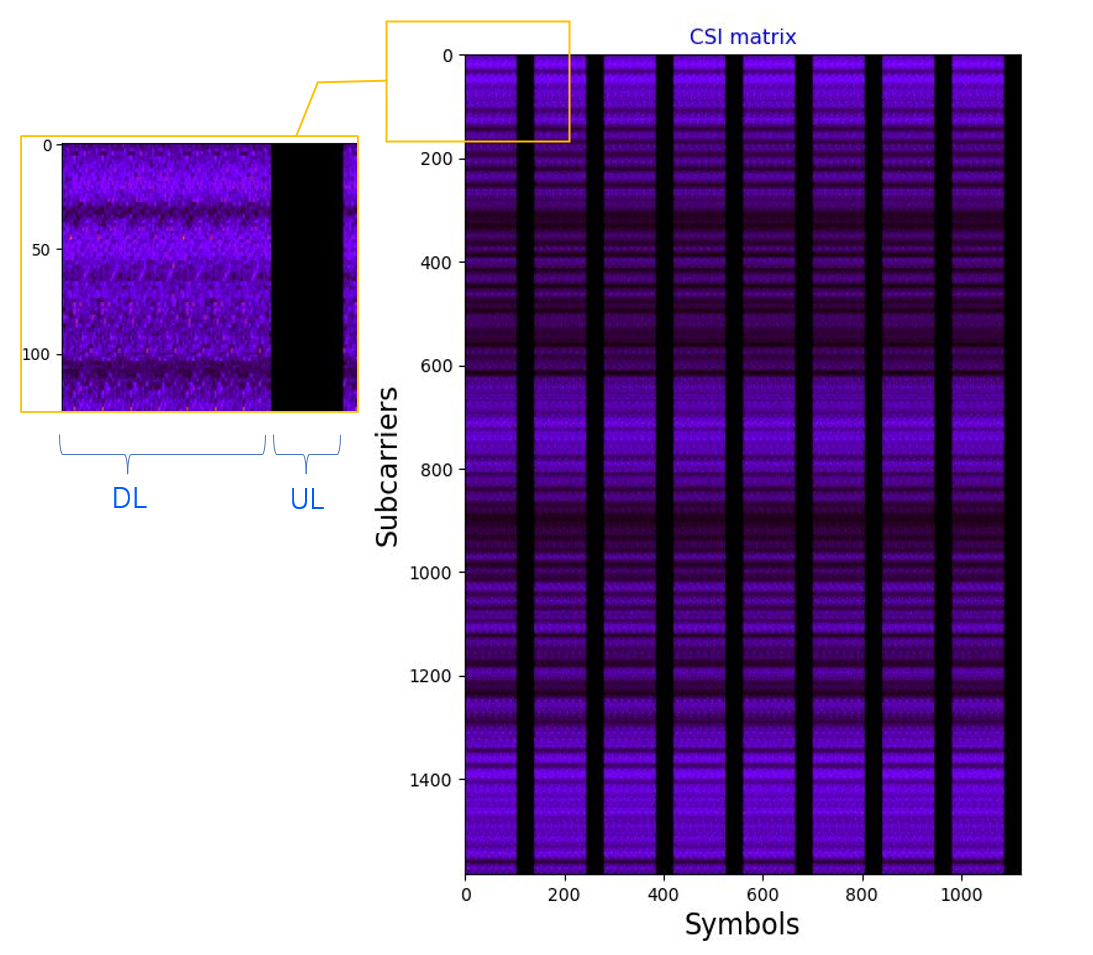
\includegraphics[width=0.5\textwidth]{Images/TDDprocessing/CSIMatrix_DLULpattern.png}
    \caption{CSI matrix from NOKIA PoC, rows and columns correspond to OFDM subcarriers and symbols respectively}
    \label{fig:CSIMatrix_DLULpattern}
\end{figure}

\section{Ideal system performance}

Without modifying the OFDM frame, the system can carry out radar processing with the following performance:

\begin{itemize}
    \item \textbf{Unambiguous speed}
     \vspace{-\baselineskip} % Remove extra whitespace
            \begin{equation}
                v_{\text{unamb}} = \frac{c_0}{2f_C T_S} = 613,15\text{ m/s}.
            \end{equation}
           
     \item \textbf{Unambiguous range}
            \begin{equation}
                d_{\text{unamb}} = \frac{c_0}{2\Delta_f} = 1250,0\text{ m}.
            \end{equation}
     \item \textbf{Speed resolution}
            \begin{equation}
                v_{\text{res}} = \frac{c_0}{2T_Sf_CM} = 0,603 \text{ m/s}.
            \end{equation} 
     \item \textbf{Range resolution}
            \begin{equation}
                d_{\text{res}} = \frac{c_0}{2\Delta_fN} = 0,789 \text{ m}.
            \end{equation}  
\end{itemize}



\section{Effect of empty UL symbols}
    
    The removal of UL symbols acts as windowing on the received frame. This introduces additional spectral replicas in speed as shown in figure \ref{fig:SpectralReplicasDLULpattern}. Replicas seem to appear at a constant speed displacement from where actual targets lie, behaving similarly to replicas due to the radar's non-ambiguity speed.
    
    \begin{figure}[H]
        \centering
        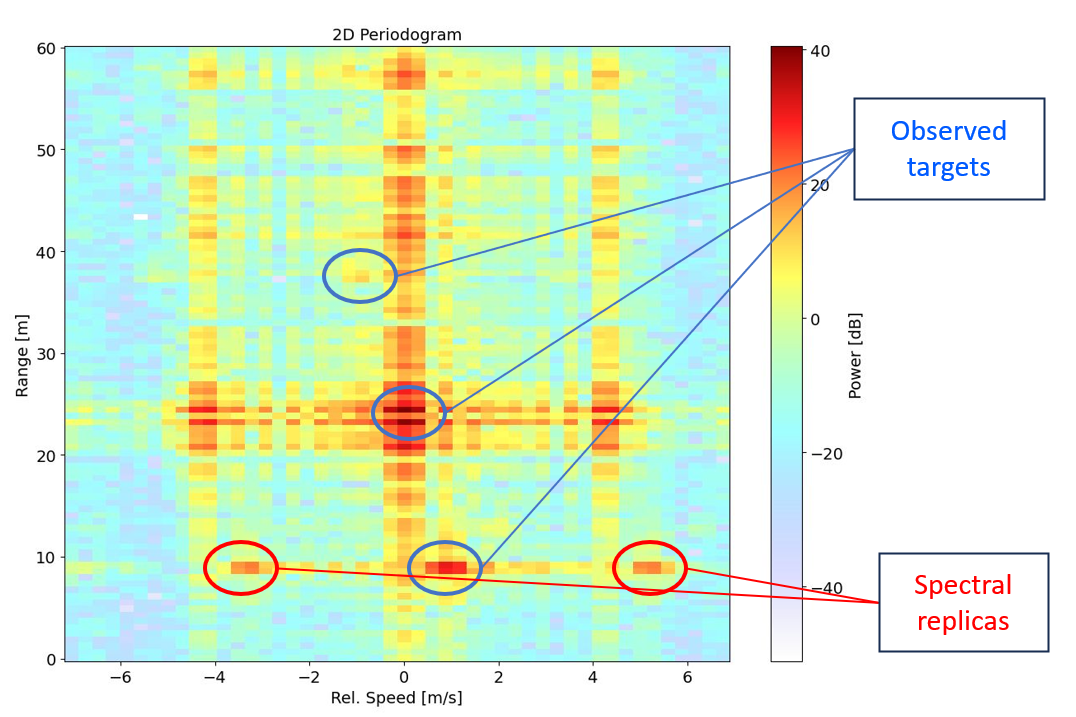
\includegraphics[width=0.55\textwidth]{Images/TDDprocessing/SpectralReplicasDLULpattern.png}
        \caption{Periodogram of a radar measurement with: static target at 23 m; moving target (range = 9,5 m, speed = 0,94 m/s); NLOS target (range = 37,2 m, speed = -1 m/s)}
        \label{fig:SpectralReplicasDLULpattern}
    \end{figure}
    
    In order to characterize the additional spectral replicas, the windowing function used to set all UL symbols to zero is analyzed. The windowing pattern can be expressed in the form
    
    \begin{align}
        &\text{rect}\left( \frac{t + \tau}{104 \cdot T_S}\right) \ast \sum_{i=0}^7 \delta\left( t - i\cdot \frac{140}{1120}\cdot T_{\text{frame}} \right),  \\
        &T_{\text{frame}} = 1120 \cdot T_S.
    \end{align}

    The windowing function, apart from a time-shift factor, is a rectangle function (Dirichlet window) convoluted with a train of Dirac deltas with spacing of 140 samples, Figure \ref{fig:TDDproc_rectfunct}. Its transform in frequency, Figure \ref{fig:TDDproc_rectfunct_transform}, is a cardinal sine function multiplied by a train of Dirac deltas.

    The transform is then convoluted with the signal in the frequency domain. The impulses adjacent to the one at zero-frequency in figure \ref{fig:TDDproc_rectfunct_transform} appear as replicas in the periodogram. These peaks have enough power to be detected as actual targets, limiting the system's performance by reducing the effective unambiguous speed or by masking actual targets that would be detected near the replica. 

\begin{figure}[H]
    \centering
    
    \subfloat[TDD windowing function\label{fig:TDDproc_rectfunct}]{%
        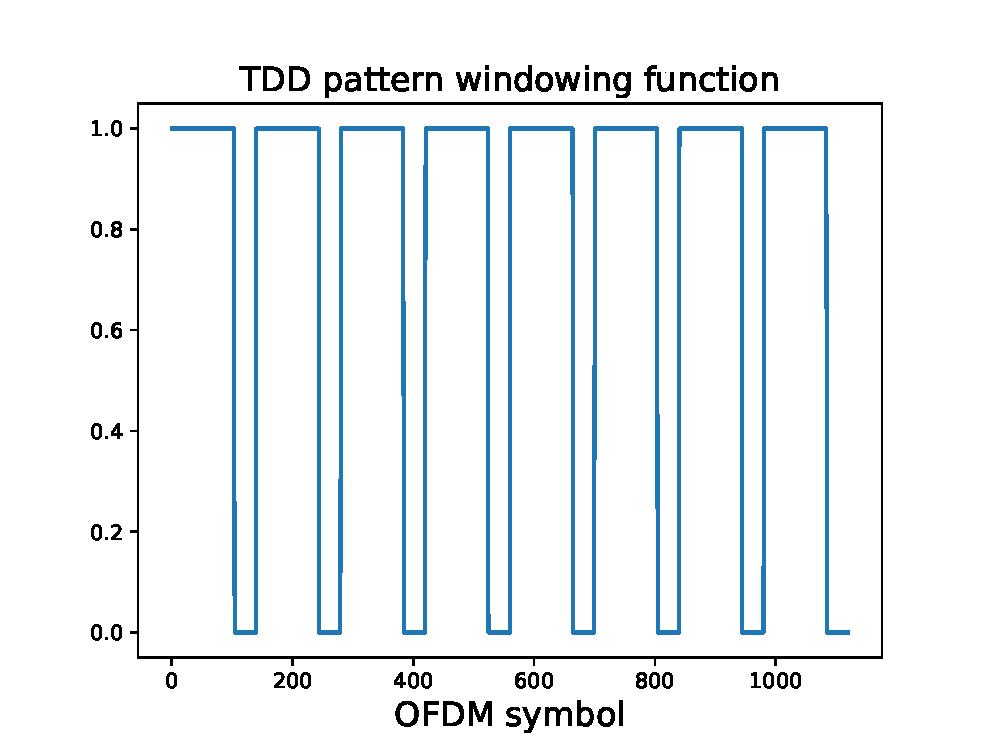
\includegraphics[scale=0.5]{Images/TDDprocessing/rectFunct.eps}%
    }\hfill
    \subfloat[Transform of the windowing function, FFT over 2048 points, absolute value\label{fig:TDDproc_rectfunct_transform}]{%
        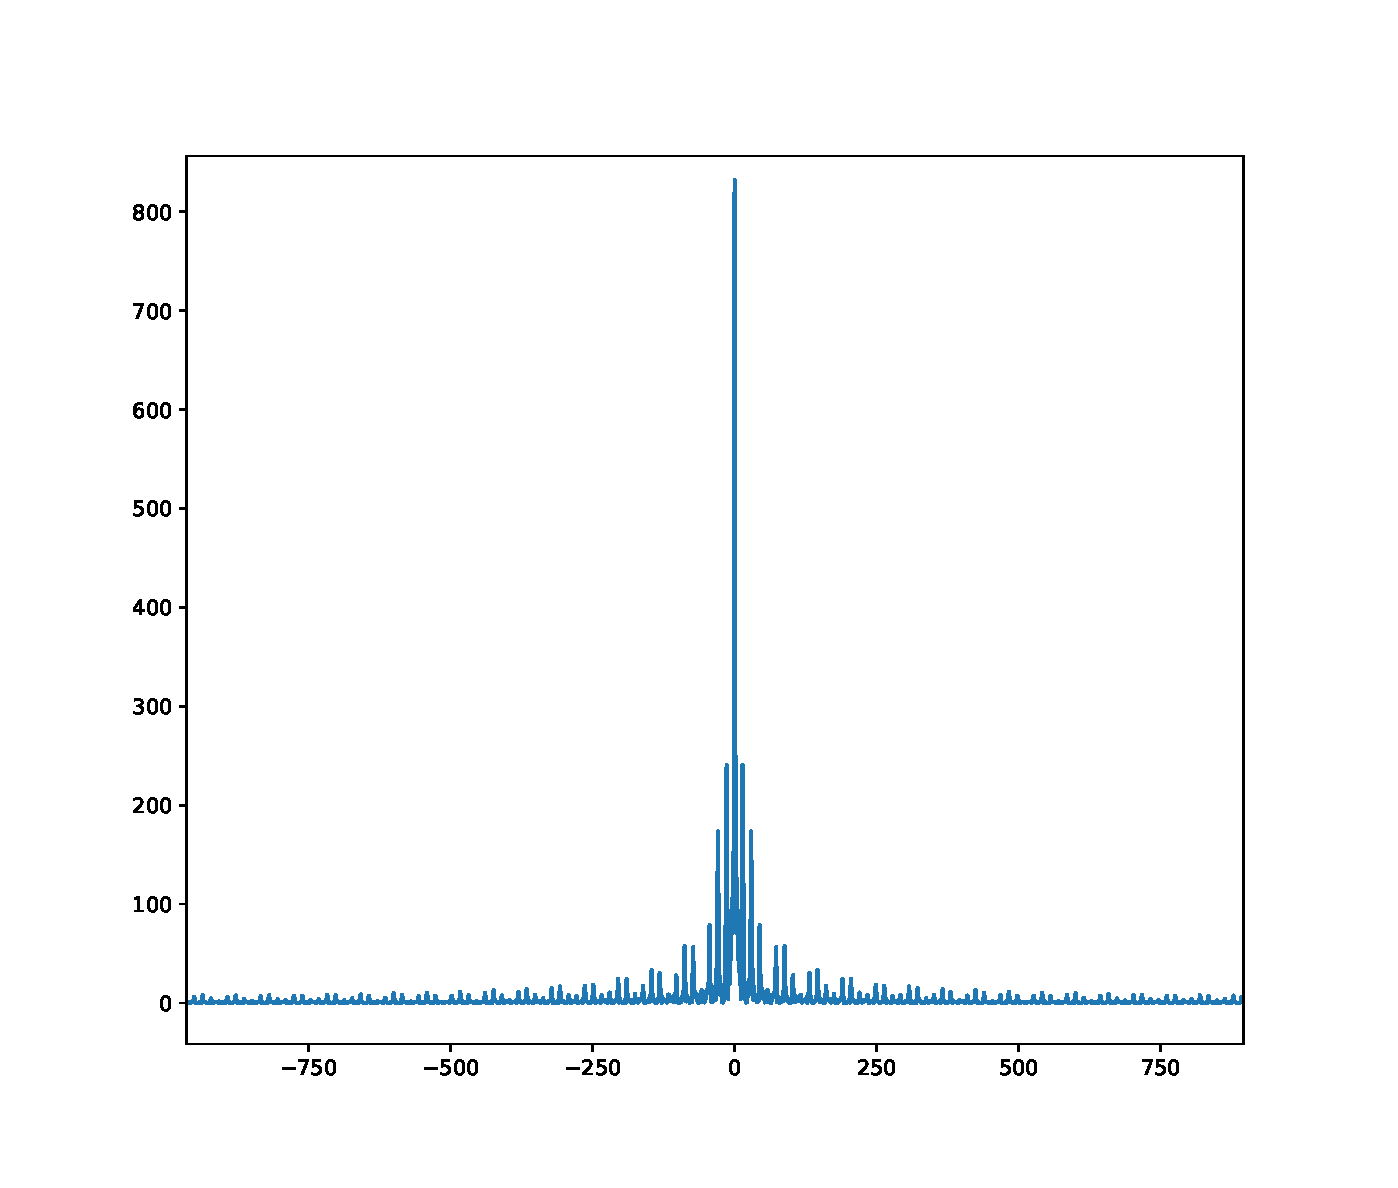
\includegraphics[scale=0.335]{Images/TDDprocessing/transform_of_rectFunct1.eps}%
    }
    
    \caption[]{}
    \label{fig:TDDwindowingfunct}
\end{figure}

\section{Frame sampling strategies}

    \begin{figure}[H]
        \centering
        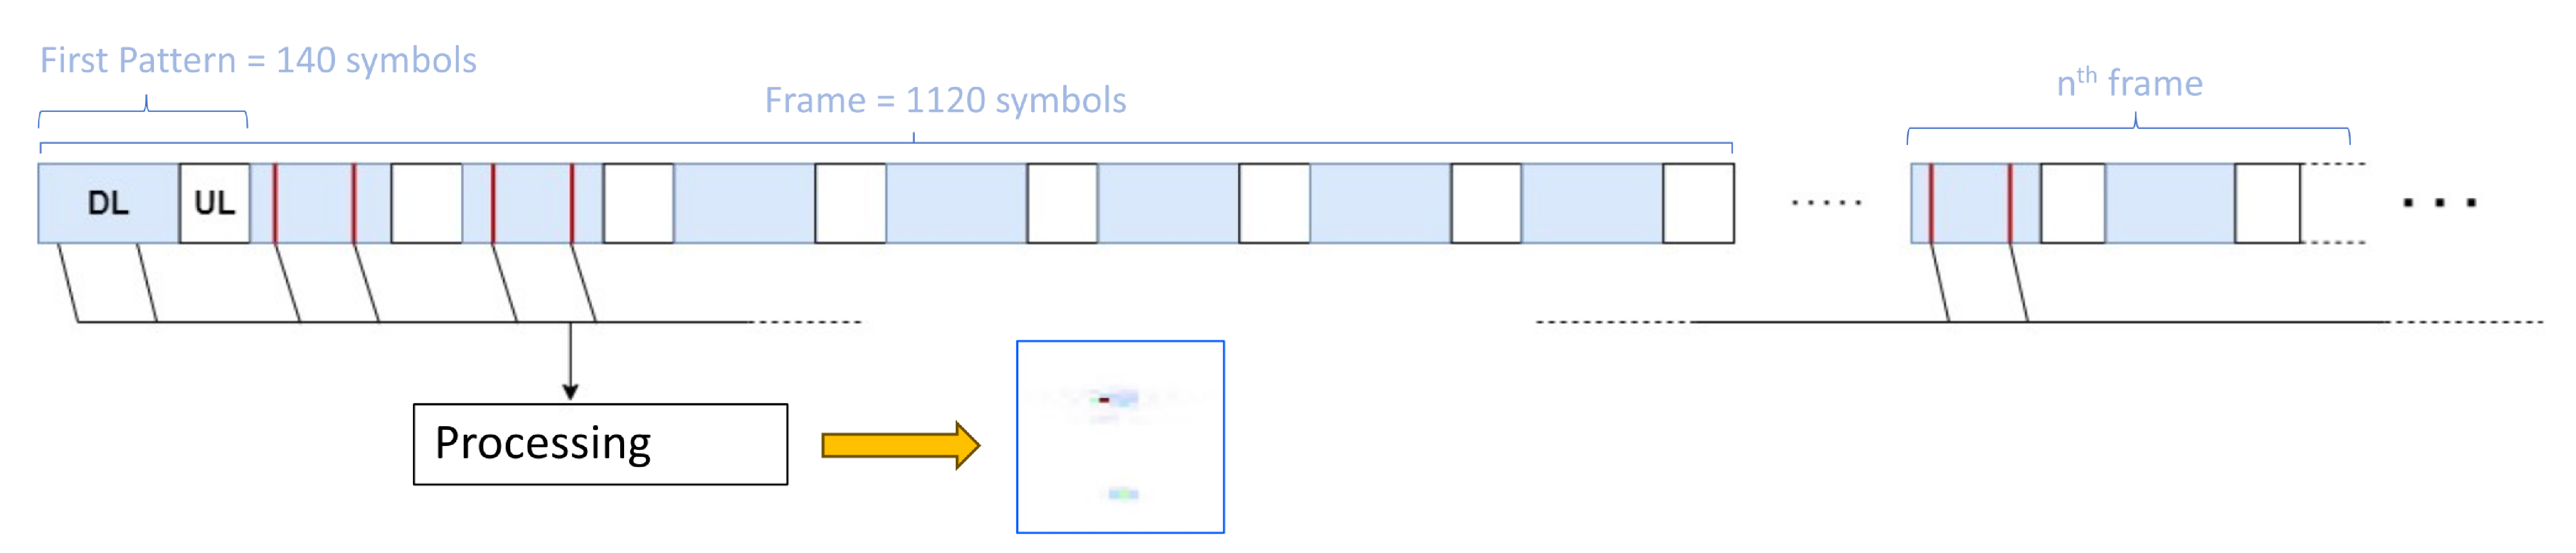
\includegraphics[width=1\textwidth]{Images/TDDprocessing/TDDstrategies.eps}
        \caption{Decimation and combining of different consecutive frames}
        \label{fig:TDDstrategies}
    \end{figure}

    \paragraph{Single DL pattern:}
    in order to avoid processing blank UL symbols, the most straightforward approach would be processing only the first 104 DL symbols. The replicas would be avoided, but the time aperture of the measure would be reduced by a factor 8, decreasing the speed resolution from $0,603$ m/s to $\approx 5,88$ m/s, unusable for most of the sensing use cases.
    
    \paragraph{Decimation at constant interval:}
     a possible strategy is re-sampling the OFDM frame in time at a fixed pace, avoiding blank symbols. Replicas are not detected, but the lower number of processed symbols translates into a considerable loss of SNR in the periodogram. This affects NLOS sensing in particular, since targets observed from a reflection present a considerably lower peak power compared with the LOS components.

     Reducing the number of available symbols with a fixed time-aperture translates in lower granularity of measurements and in a decrease in unambiguous speed. \protect\newline In the case of Figure \ref{fig:TDDperiodogram1FYesDec}, processing one symbol every 47, the obtained unambiguous speed is $13,05$ m/s. \protect\newline Speed resolution remains unchanged.
    
     \paragraph{Decimation and multi-frame processing:}
     combining consecutive frames, it is possible to process an higher number of symbols, re-gaining a part of the SNR thanks to processing gain, all without observing replicas. The time aperture of the measurement is also increased, translating into a better speed resolution.

     This approach introduces a trade-off between SNR (processing gain) and update rate. Increasing the time-aperture, some range migration effect can be observed, especially for fast moving targets. In the context of NLOS sensing, the impact of range migration on system performance is relatively minor compared to the benefits of increased speed resolution and higher signal-to-noise ratio, since the primary goal is not providing precise tracking or positioning data.


    In Figures \ref{fig:TDDperiodogram1FNoDec}-\ref{fig:TDDperiodogram10frames} it is possible to observe the effects of the various strategies when applied to a OFDM radar measurement where both the NLOS and LOS components are present for a single target.


% 2x2 figure scheme
    \begin{figure}[H]
        \centering
        
        \subfloat[Single processed frame, no decimation, SNR = 60,91 dB, \protect\newline $v_{\text{res}} = 0,603$ m/s, $ v_{\text{unamb}} = 613,15$ m/s
\label{fig:TDDperiodogram1FNoDec}]{
            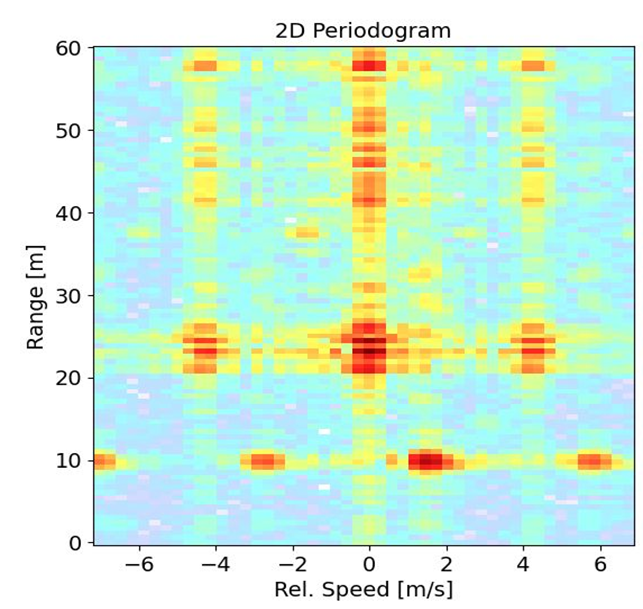
\includegraphics[width=0.4\textwidth]{Images/TDDprocessing/periodogram1FNoDec.png}
        }
        \hfill
        \subfloat[Single processed frame, decimated, \protect\newline SNR = 45,16 dB, \protect\newline $v_{\text{res}} = 0,603$ m/s, $ v_{\text{unamb}} = 13,05$ m/s\label{fig:TDDperiodogram1FYesDec}]{
            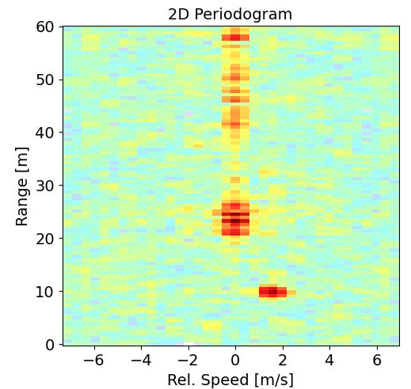
\includegraphics[width=0.4\textwidth]{Images/TDDprocessing/periodogram1FYesDec.png}
        }
        
        \vspace{0.5cm}
        
        \subfloat[6 processed frames, decimated, combined, SNR = 52,35 dB, \protect\newline $v_{\text{res}} = 0,091$ m/s, $ v_{\text{unamb}} = 8,76$ m/s\label{fig:TDDperiodogram6frames}]{
            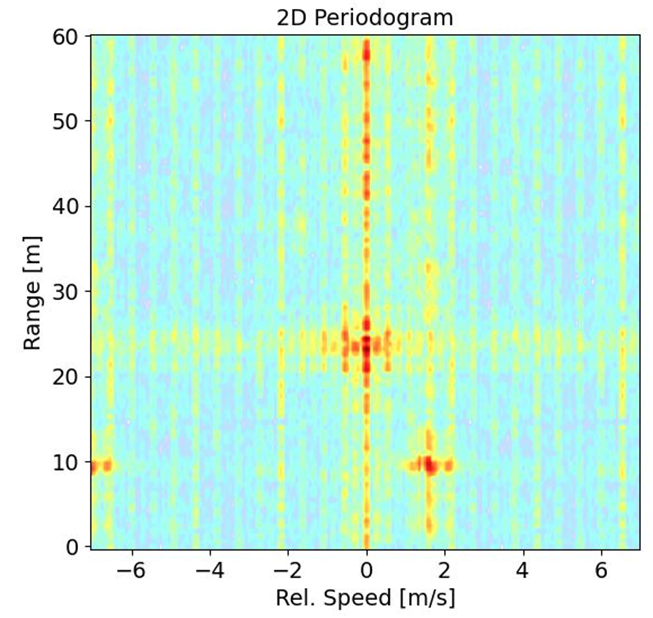
\includegraphics[width=0.4\textwidth]{Images/TDDprocessing/periodogram6frames.png}
        }
        \hfill
        \subfloat[10 processed frames, decimated, combined, SNR = 54.66 dB, \protect\newline $v_{\text{res}} = 0,054$ m/s, $ v_{\text{unamb}} = 8,76$ m/s\label{fig:TDDperiodogram10frames}]{
            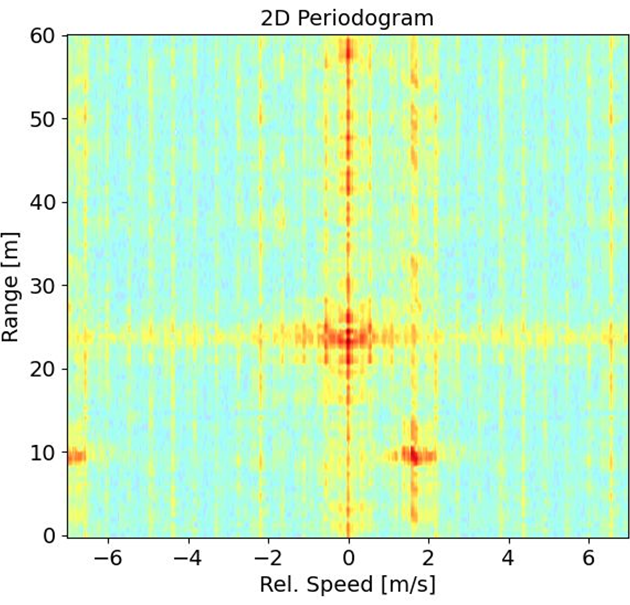
\includegraphics[width=0.4\textwidth]{Images/TDDprocessing/periodogram10frames.png}
        }
        
        \caption{Examples of possible decimation and combining approaches in periodogram processing}
        \label{fig:allperiodogram-decimation}
    \end{figure}


    
\begin{table}[H]
    %\caption*{\textbf{Title of Table (optional)}}
    \centering 
    \begin{tabular}{|p{9em} c c c |}
    \hline
    \rowcolor{bluepoli!40} % comment this line to remove the color
     \textbf{Strategy} & \textbf{SNR [dB]} & \textbf{N} & \textbf{Time aperture [ms]} \T\B \\
    \hline \hline
    $\textbf{Standard frame}$ & 60,91 & 1120 & 10 \T\B \\
    $\textbf{Decimated frame}$ & 45,16 & 24 & 10 \T\B\\
    $\textbf{6 frames}$ & 52,35 & 96 & 60  \T\B\\
    $\textbf{10 frames}$ & 54,66 & 160 & 100  \T\B\\

    \hline
    \end{tabular}
    \\[10pt]
    \caption{Comparison between SNR levels for different frame processing strategies}
    \label{table:TDDstratcomparison}
\end{table}



% Radar detection and thresholding techniques
% !TeX spellcheck = <none>
\chapter{Radar frame processing}
\label{chap:radar_detection}

\section{Radar search and detection}
Detection is commonly defined as the process of analysing the radar data and determining whether it consists of noise only, or noise plus echoes coming from a target of interest \cite{Richards_Scheer_Holm_2010}. 
The first hypothesis is denoted as the null hypothesis $H_0$ and the second as the non-null hypothesis $H_1$.
Detection is achieved by setting a threshold for the region of interest, based on the level of interference, and deciding whether any part of that region is "bright" enough compared to the background.

%TODO generate image showing fixed vs adaptive threshold

Radar users are typically concerned with determining (or defining) the probability of detecting a target $P_D$ and the probability of false alarm $P_{FA}$.  By utilizing the knowledge of the desired $P_{FA}$, noise statistics, and detector design, it is possible to decide the appropriate threshold level to be used at the detector's output.

% TODO asses feasibility of confirmation system (does not work for clutter)



% TODO consider putting something about clutter statistics

In this work different approaches were be considered and their respective advantages and drawbacks analysed. 



\subsection{Constant False Alarm Rate}
	
	Standard radar detection assumes the level of noise and interference to be known and constant. In this conditions it is possible to precisely determine the correct threshold for achieving the desired $	p_\text{FA}$. In real scenarios interference levels may be highly variable throughout an acquisition, making the use of a dynamic threshold necessary. Constant false alarm rate (CFAR) is an adapting threshold technique aiming at providing predictable behaviour of detection and false alarm rates in real scenarios.
	
	%TODO generate image showing fixed vs adaptive threshold
	
	In OFDM radar, a \textit{false alarm} occurs when the target detector determines the presence of a target at a range and relative speed that does not contribute to the received matrix $\bm{F}_{Rx}$ \cite{Braun2014OFDMRA}. 
	Consequently, the probability of false alarm is the probability of observing a positive detection when the received frame consists only of noise $(\bm{F}_{Rx} = \bm{Z})$. 
	This definition considers processing on a per-frame basis and can also be applied to the multi-frame processing strategies presented in chapter \ref{chap:TDD pattern of the OFDM frame}. 
	
	The presence of clutter is not yet taken into account as the threshold is estimated by determining an estimator for the noise power of the processed data. 
	Furthermore, clutter can be defined as reflections generated by objects in the environment, that are not of interest for the sensing task. 
	This means that detections due to objects considered as clutter are expected and can be mitigated by various clutter removal techniques.
	
	In order to discriminate noise from signal power, the periodogram is subjected to an hypothesis test with an appropriate threshold
	
	\begin{align}
		\text{Per}_{\bm{F}}(n,m) \quad\mathop{\gtrless}_{H_1}^{H_0}  \quad \eta,
	\end{align}
	
	where $H_0$ is the null hypothesis, target not present, and $H_1$ is the hypothesis where the reflection from a target contributes to the received power in the bin under test.\\
	The probability that any bin of the periodogram exceeds the threshold when only noise power $Z$ is present is
	
	\begin{align}
		p_{\text{FA},bin} = \text{Per}(Z > \eta) = \int_\eta^{\infty} f_z(z|H_0)dz = 1 - F_z(\eta | H_0) = e^{-\dfrac{\eta}{\sigma_n^2}},
	\end{align}
	 
	where $f_z(z|H_0)$ and $F_z(\eta | H_0)$ are the PDF and CDF of the random variable $Z$. 
	The observed noise contribution is given by the magnitude squared of the AWGN with power $\sigma_n^2$.
	 
	The threshold for a given false alarm rate per bin is obtained as
	
	\begin{align}
		\eta = -\sigma_n^2 \ln(p_{\text{FA},bin}) .
	\end{align} 
	
	Optimality for this detection method and a more thorough theoretical analysis can be found in chapter 15 of \cite{Richards_Scheer_Holm_2010}.
	For the full (non zero padded) periodogram the false alarm probability is
	
	\begin{align}
		p_\text{FA} = 1 - (1 - p_{\text{FA},bin})^{NM}.
	\end{align}
	
	Solving this for $p_{\text{FA},bin}$ we obtain the value of the threshold as 
	
	\begin{align}
		\eta = \sigma_N^2 \ln{(1 - (1 - p_{\text{FA},bin})^{NM})}.
	\end{align}
	
	Zero padding the periodogram does not add information useful for the target estimation problem, but it only reduces quantization noise. The contribution of a single bin is spread out between multiple contiguous bins when zero padding.

	\subsubsection{Estimation of noise power}
	
		Noise power is estimated from the periodogram averaging over bins where the target is not expected.
		
		From Assumption 3 from section \ref{sub:assumptions_ofdm_radar}, the maximum target delay and consequently the maximum range bin in which we can observe a target depend on the guard interval defined by the CP, and are given by
		\begin{align}
			\tau_{\text{max}} =& \frac{N_{\text{max}}}{N_{\text{Per}}}\cdot T = T_\text{CP} ,\\
			N_{\text{max}} =& \frac{T_\text{CP}}{T}\cdot N_{\text{Per}}.
		\end{align} 
		
		The maximum likelihood estimate for the noise power is found by averaging over one or more rows beyond $N_{\text{max}}$

		\begin{align}
		\label{align: threshold_noise_power}
			\hat{\sigma_N}^2 = \frac{1}{M_{\text{Per}}K} \sum_{k=1}^K \sum_{m=1}^{M_{\text{Per}}} \text{Per}_{\bm{F}}(N_{\text{max}}+k, m).
		\end{align}

Standard CFAR is an established method, howeverit was observed that estimating a fixed threshold across the periodogram based only on the level of the noise floor leads numerous above-threshold cells due to the sidelobes of the target returns, as shown in Figure \ref{fig:RadThesh_CFAR_abv_thresh_doubl}.

	\begin{figure}[H]
	\centering
	
	\subfloat[Above-threshold bins, threshold estimated using CFAR.\label{fig:RadThesh_CFAR_abv_thresh}]{%
		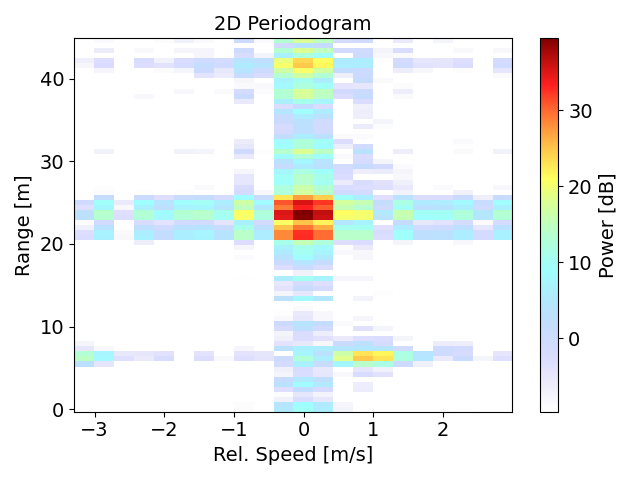
\includegraphics[scale=0.45]{Images/radar_detect_threshold/cfar_abv_thresh.png}%
	}\hfill
	\subfloat[Reference periodogram. \label{fig:RadThesh_CFAR_abv_thresh_PER}]{%
		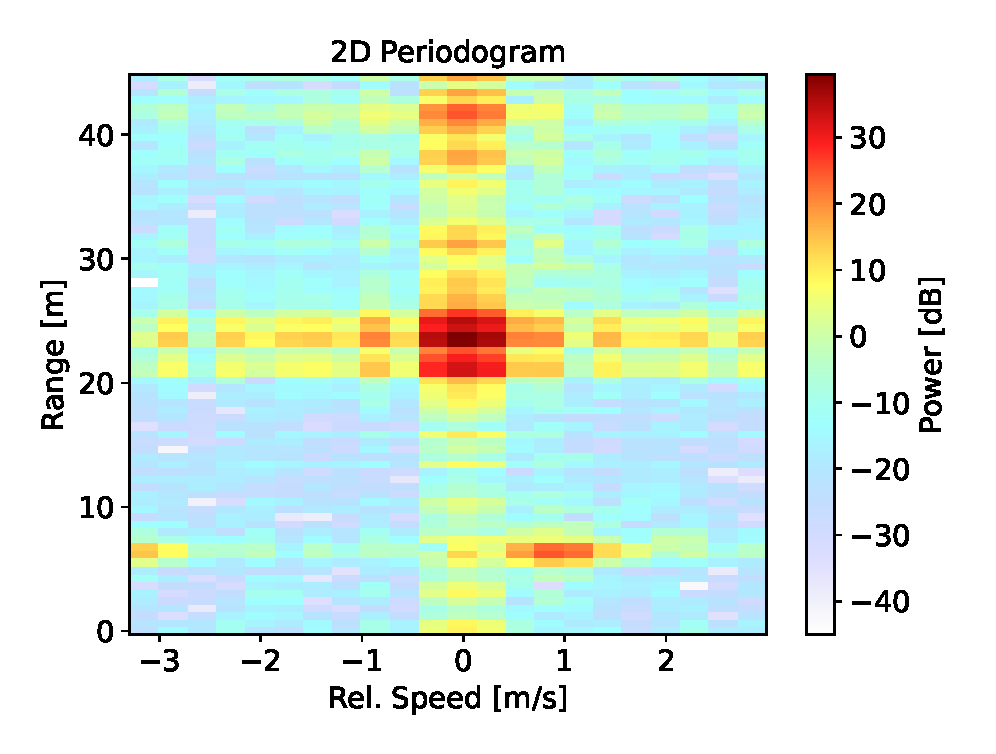
\includegraphics[scale=0.45]{Images/radar_detect_threshold/cfar_abv_thresh_PER.eps}%
	}
	
	\caption[]{Example of CFAR thresholding, it can be observed that the largest target positioned at 23 m (a wall) presents strong sidelobes that are detected as target returns.}
	\label{fig:RadThesh_CFAR_abv_thresh_doubl}
\end{figure}


One common method for significantly reducing false alarms after the detection process is using a confirmation system that requires each target to be detected twice: once in the initial search and in a subsequent confirmation process.
However, there is still the possibility that a noise spike will remain in the confirmation measure and the target will not. In addition, this approach can suffer from peaks generated by clutter or spectral artefacts that may persist over time.

\subsection{Cell-averaging CFAR}
\label{sec:cell averaging CFAR}

The generic CFAR detector described in the previous section defines a threshold, based on noise power, to be applied to the whole periodogram. More advanced algorithms for CFAR detection belong to the family of cell-averaging CFAR (CA-CFAR) \cite{Richards_2014}.

In a noisy environment, very weak echo signals may be lost in the case of a fixed threshold across the periodogram. CA-CFAR estimates the threshold level for each cell of the 2D periodogram based on the statistics of neighbouring cells belonging inside a set reference window. In this way noise levels are estimated for smaller sections of the periodogram, adapting to the level of the noise floor and defining a variable treshold across the periodogram.

The CFAR window resides inside the data window and is composed of leading and lagging reference windows, guard cells and cell-under-test (CUT). Guard cells are discarded for noise computation since they may contain returns associated with the target in the CUT.

In the OFDM range-doppler radar problem a two-dimensional CFAR window is considered, where the CUT is located at the center.

\begin{figure}[H]
	\centering
	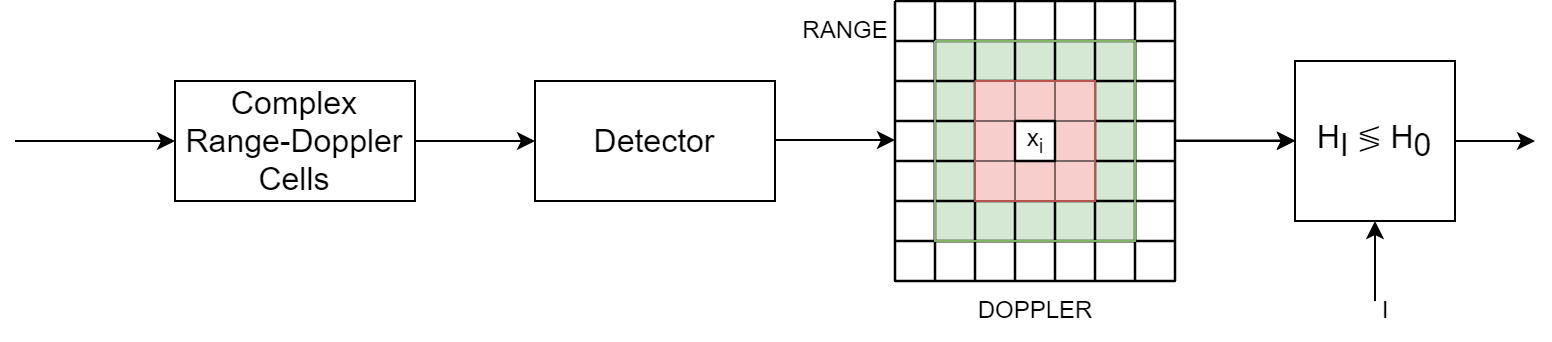
\includegraphics[width=0.9\textwidth]{Images/radar_detect_threshold/cacfar_pipeline.png}
	\caption{CA-CFAR detection processor, guard cells are indicated in red, while reference cells are highlighted in green.}
	\label{fig:cacfar_pipeline}
\end{figure}


% TODO: insert CACFAR scheme from presentation (add guard cells)
% TODO: insert sliding windows

The CA-CFAR threshold is defined by the product of the noise power estimate and a CFAR constant

\begin{align}
	T = \alpha_{\text{CA}} \hat{\sigma_N}^2.
\end{align}

The CFAR constant $\alpha_{\text{CA}}$ is a function of the probability of false alarm $p_{\text{FA}}$ and of the number of contribution cells $N$ and is derived as in chapter 16.5 of \cite{Richards_Scheer_Holm_2010}. The estimated noise power is calculated as in \ref{align: threshold_noise_power} by averaging over the contributing cells

\begin{align}
	\alpha_{\text{CA}} =& N[p_{\text{FA}}^{-1/N} - 1] \\
	\hat{\sigma_N}^2 =& \frac{1}{N}\sum_{n=1}^N z_n.
\end{align}

The number of operations can be reduced by simplifying the normalization by $\frac{1}{N}$ by defining a noise statistics $\hat{g}_{\text{CA}}' = \sum_{n=1}^N z_n$ and by incorporating it in the CFAR constant $\alpha_{\text{CA}}' = p_{\text{FA}}^{-1/N} - 1$.

Computationally CA-CFAR is more demanding than other thresholding techniques, as in its fastest implementation it still requires a 2D convolution to be applied to the periodogram before computing the threshold at each bin.

\subsubsection{Performance of CA-CFAR}

The general assumption that each radar return occupies one single bin in the range-Doppler plane is not valid for OFDM radar systems, as the PSF is influenced by a number of factors.
Zero padding and windowing in the periodogram define the width of the main lobe of the sinusoids in the 2D plane, while a large time aperture of the acquisition generally leads to a larger return due to range and Doppler spreading.

In a heterogeneous radar frame multiple targets and changes in the interference power degrade CFAR performance. If target returns are present in the reference window, they will bias the threshold and lead to a missed detection. This phenomenon is called \textit{target masking}. Another source of performance degradation is the presence of clutter, where \textit{clutter boundaries} are zones in which there is a sudden change in the statistics of the interfering power.

Performance is also strongly influenced by the design of the reference window. The window should be designed to be as small as possible, in order to reduce the computational load due to the convolution operation and not to include interfering statistics far away from the CUT. The guard interval should be dimensioned according to the point spread function of the target return. An extended target could be counted in the reference window and lead to \textit{self masking}.

	\begin{figure}[H]
		\centering
		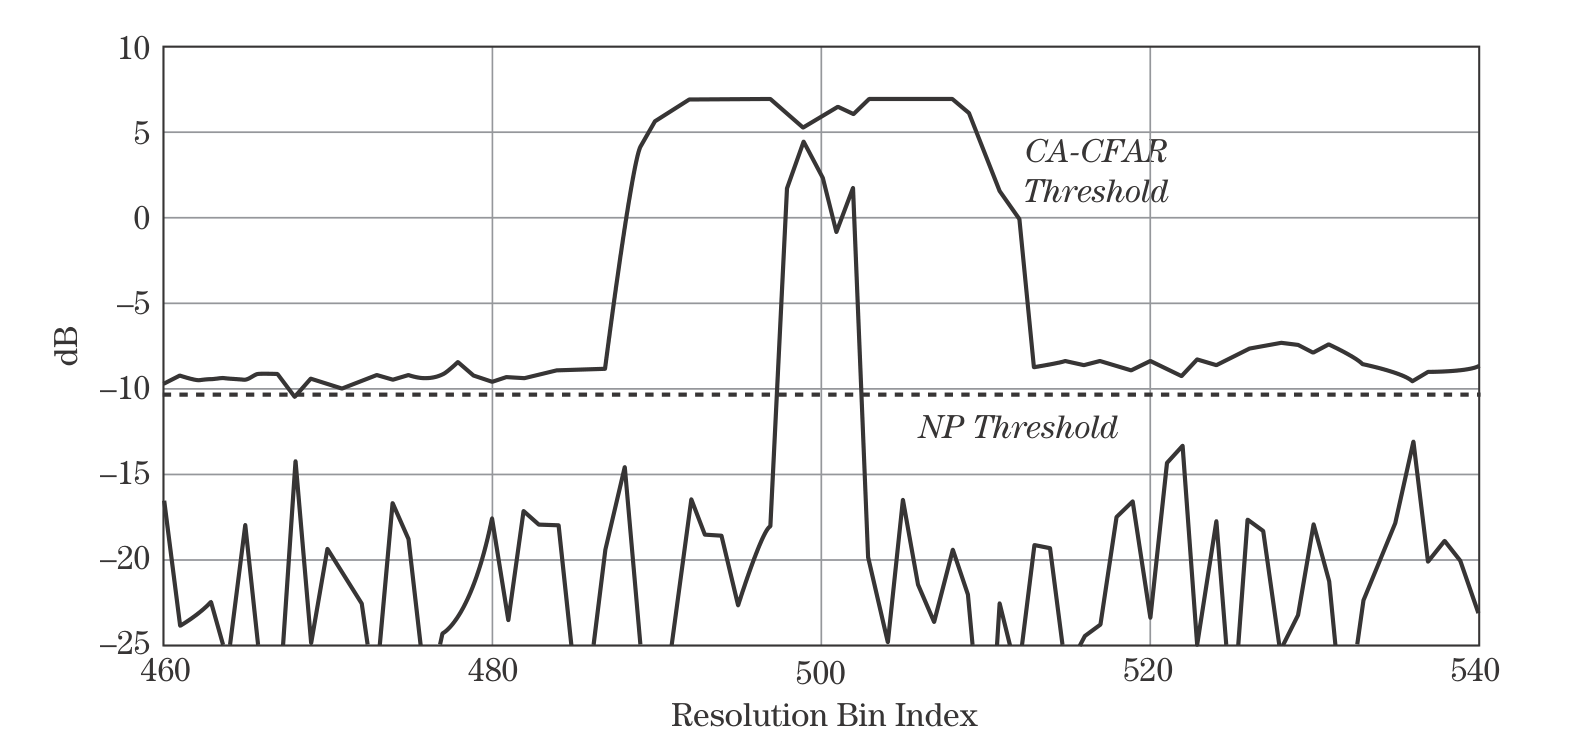
\includegraphics[width=0.7\textwidth]{Images/radar_detect_threshold/self_masking_Richards2010.png}
		\caption{Example of self masking in a 1D radar signal \cite{Richards_Scheer_Holm_2010}}
		\label{fig:self_masking_Richards2010}
	\end{figure}

	\begin{figure}[H]
		\centering
		
		\subfloat[Above-threshold bins using CA-CFAR.\label{fig:RadThesh_CA_CFAR_missed_detect}]{%
			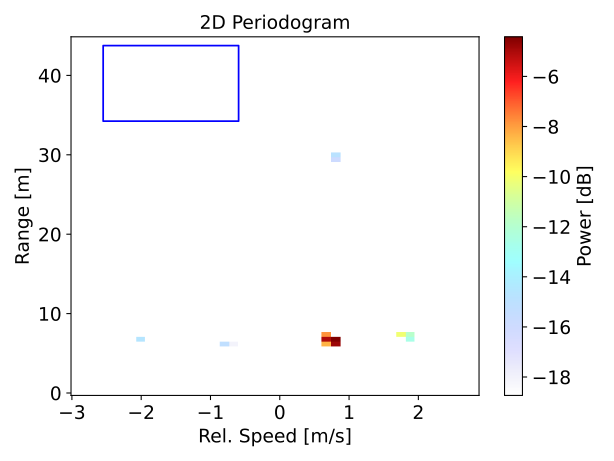
\includegraphics[scale=0.45]{Images/radar_detect_threshold/ca_cfar_no_nlos_1.png}%
		}\hfill
		\subfloat[Reference periodogram. LOS target at 6 m and corresponding NLOS path return at 40 m, -1,5 m/s.\label{fig:RadThesh_CA_CFAR_missed_detect_PER}]{%
			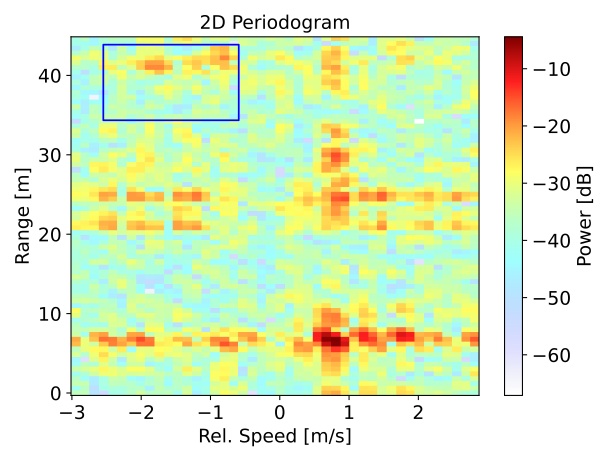
\includegraphics[scale=0.45]{Images/radar_detect_threshold/ca_cfar_no_nlos_PER_1.png}%
		}
		
		\caption[]{Clutter-like return observed in NLOS (top-left area denoted by the blue box): CA-CFAR uses part of the point cloud to estimate noise levels and the target is not detected.}
		\label{fig:RadThesh_CA_CFAR_missed_detect_doubl}
	\end{figure}

	In a NLOS sensing scenario, CA-CFAR suffers from these drawbacks due to the lower SNR of target returns caused by multiple reflections and the presence of strong clutter components close to the zero-doppler bin. 
	Additionally, as NLOS returns propagate over a larger distance their PSF in the periodogram can assume a form similar to clutter. 
	As a result, they do not appear as distinct peaks, but rather are spread across neighbouring bins, which raises the CA-CFAR threshold and leads to missed detections, as shown in Figure \ref{fig:RadThesh_CA_CFAR_missed_detect_doubl}.

\subsubsection{Robust CA-CFAR}
More complex CA-CFAR algorithms may provide better results under certain heterogeneous conditions, but at the expense of increased computational complexity, higher cost, or lower performance under non-ideal conditions.

Some of the more common variations of the algorithm are the greatest-of CA-CFAR (GOCA-CFAR) and the censored statistics CA-CFAR (CSCA-CFAR), which are designed to suppress clutter-edge false alarms and mutual target masking, respectively.

\paragraph{Greatest-of CA-CFAR:}
the interference power is calculated in the lagging and leading reference windows separately and the largest of the two is selected as the reference statistics. In the OFDM radar signal the leading/lagging definition can be applied only in the doppler dimension, since interference statistics is assumed homogeneous in range.

For the purpose of moving target detection in NLOS clutter-edge false alarms are not a real issue, since bins at zero-doppler are not processed.
 The main problem is given by masking due to the presence of spectral artifacts or clutter.
 
 
\paragraph{Censored-statistics CA-CFAR:}
this algorithm considers the largest $N_c$ samples to be containing returns from interfering targets, and therefore does not consider them when computing the interference statistics. CSCA-CFAR is in general assumed to be capable of removing up to $N_c$ interfering targets.
This algorithm can be also generalised by censoring an arbitary number of samples in order to be adapted to different environments. 

The main limitation posed by this algorithm is the increased computational cost due to the necessary ordering of the interference samples.


\subsection{Range-adjusted exponential threshold}

	
	In \cite{Wagner_Feger_Stelzer_2017}, a different approach to thresholding was proposed for detecting large point clouds of radar returns in the 2D range-Doppler plane. Similar to the OFDM radar case, due to the relatively high speed resolution, returns occupy multiple cells in the periodogram and are not correctly detected by CA-CFAR.
	
	The idea is to adjust the threshold level accounting for the propagation loss of the target reflection, which is proportional to the square of the distance from the transmitter. 
	
	This solution was implemented combining the CFAR threshold, set as a lower bound, and the range-dependent exponential adjustement.
	
	\begin{align}
		\eta_{\text{exp}} = \eta_{\text{CFAR}} + \frac{\alpha}{d^2},
	\end{align} 
	
	where $\alpha$ is an adjustment factor for the exponential term. For this particular implementation it was defined as the square root of the maximum return in the periodogram
	
	\begin{align}
		\alpha = \sqrt{\max{ \left\{\text{Per}_{\bm{F}}(n,m)\right\} }}.
	\end{align}
	
	
	Target can then be detected by searching for local peaks in the areas above threshold. A more refined result can be obtained by applying clustering algorithms such as DBSCAN.

\section{Clutter removal}
\label{sec:clutter_removal}

	Clutter removal in radar systems refers to the process of mitigating or eliminating unwanted signals or interference that arise from various sources (such as terrain, sea, or atmospheric conditions) and can obscure the detection of true radar targets.
	In general it is possible to refer clutter as any unwanted reflection from targets that are not of interest for the radar scope.
	
	In this work two implementations of clutter removal algorithms were applied to the CSI matrix.
	Both of them work by projecting the signal into a subspace orthogonal to the clutter.
	
	Both algoritms make use of an offline clutter acquisition step, performed before the sensing task. This step is used to gather information about clutter to be removed at runtime.
	
	\paragraph{Extensive Cancellation Algorithm by Subcarrier (ECA-C):}
	This algorithm, described in \cite{Wan_Cheng_Gong_Zhao_Shao_2012}, applies ECA \cite{Colone_ECA_2009} on each subcarrier of the CSI matrix.
	This approach is successful in removing the static clutter from the periodogram, at the cost of losing information on static targets and applying some distortion to targets moving at low speed.
	
	
	\paragraph{Clutter Removal with Acquisitions Under Phase Noise (CRAP):}
	CRAP introduces a novel approach by vectorizing the CSI matrices and preserving all information in both domains, unlike ECA-C which only works on each subcarrier separately and focuses solely on the time domain of the signal \cite{Henninger_CRAP_2023}.
	
	A detailed comparison between the two approaches can be seen in Figure \ref{fig:Rad_clutter_crap-ecac}. CRAP is able to remove static clutter without distorting the position of the target.

	\begin{figure}[H]
		\centering
		
		\subfloat[\footnotesize no clutter removal, static metal target at range of ca. 10 m. Clutter at ca. 23 m.\label{fig:Rad_crap_ecac_base_static}]{%
			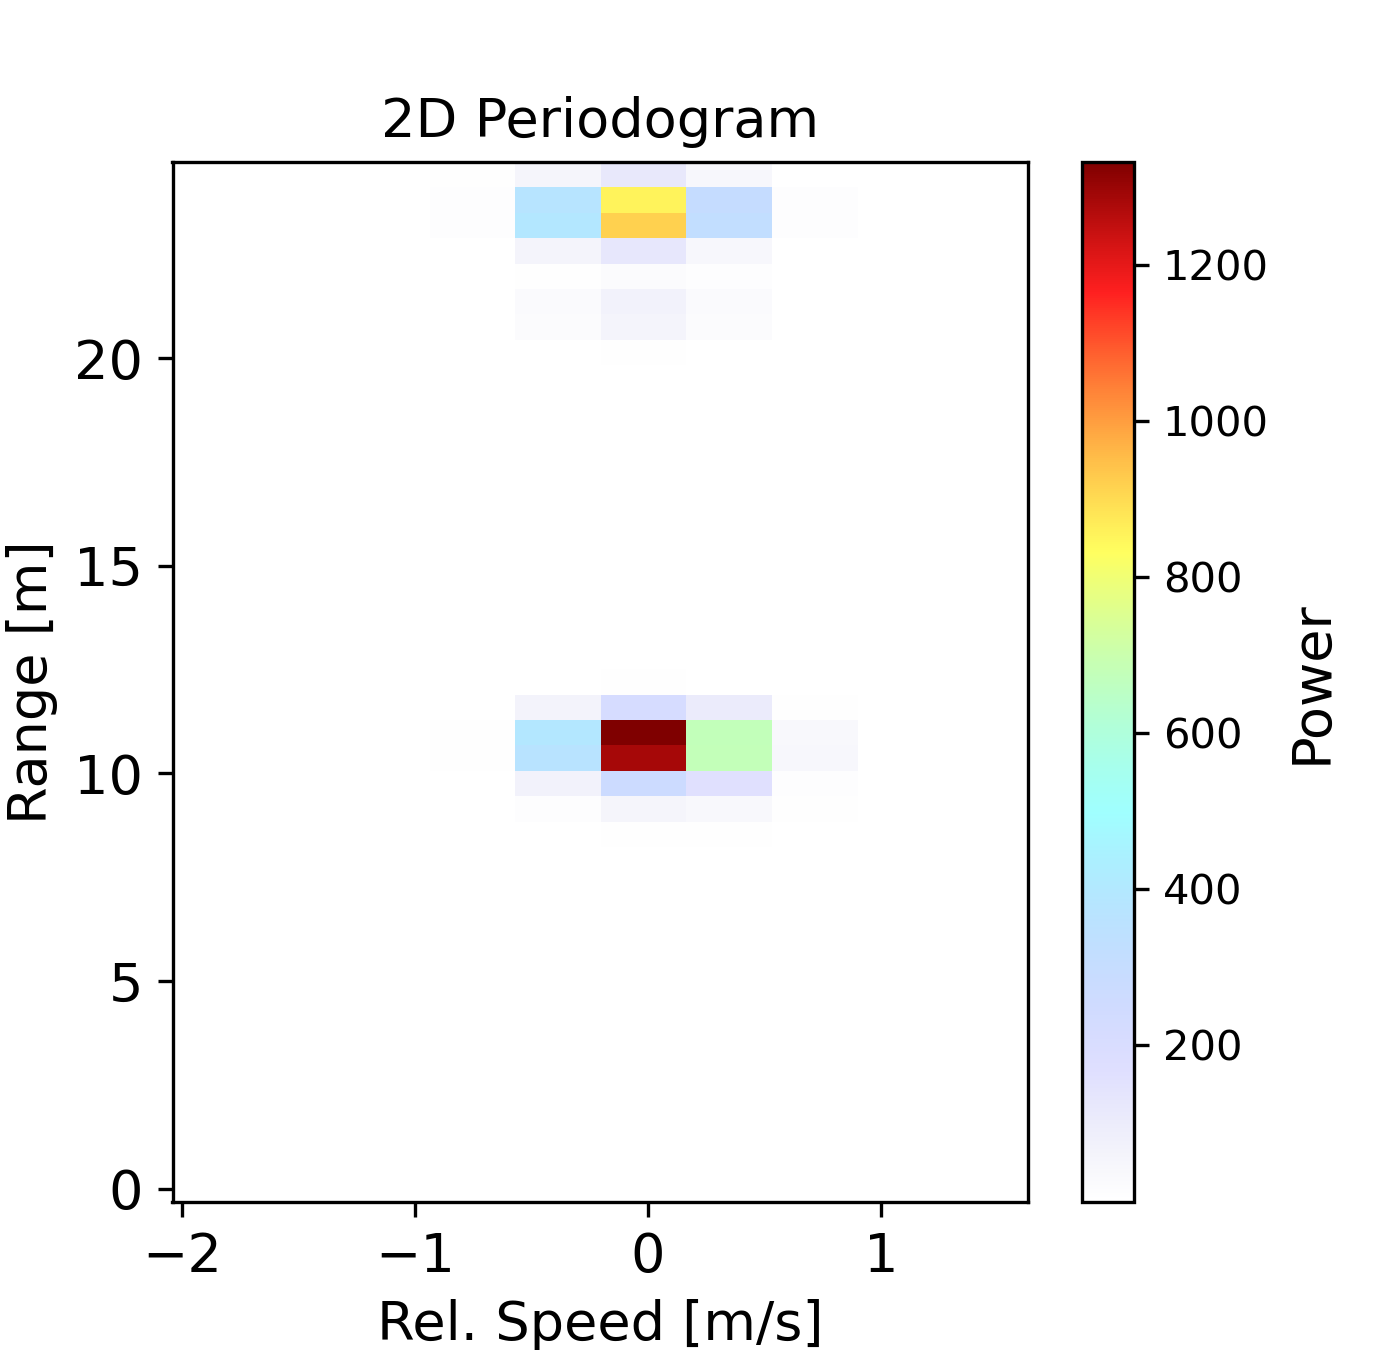
\includegraphics[scale=0.4]{Images/radar_detect_threshold/clutter/crap_ecac_static/clutter_baseline1.png}%
		}\hfill
		\subfloat[\footnotesize clutter removal with \newline ECA-C.\label{fig:Rad_crap_ecac_ECAC_static}]{%
			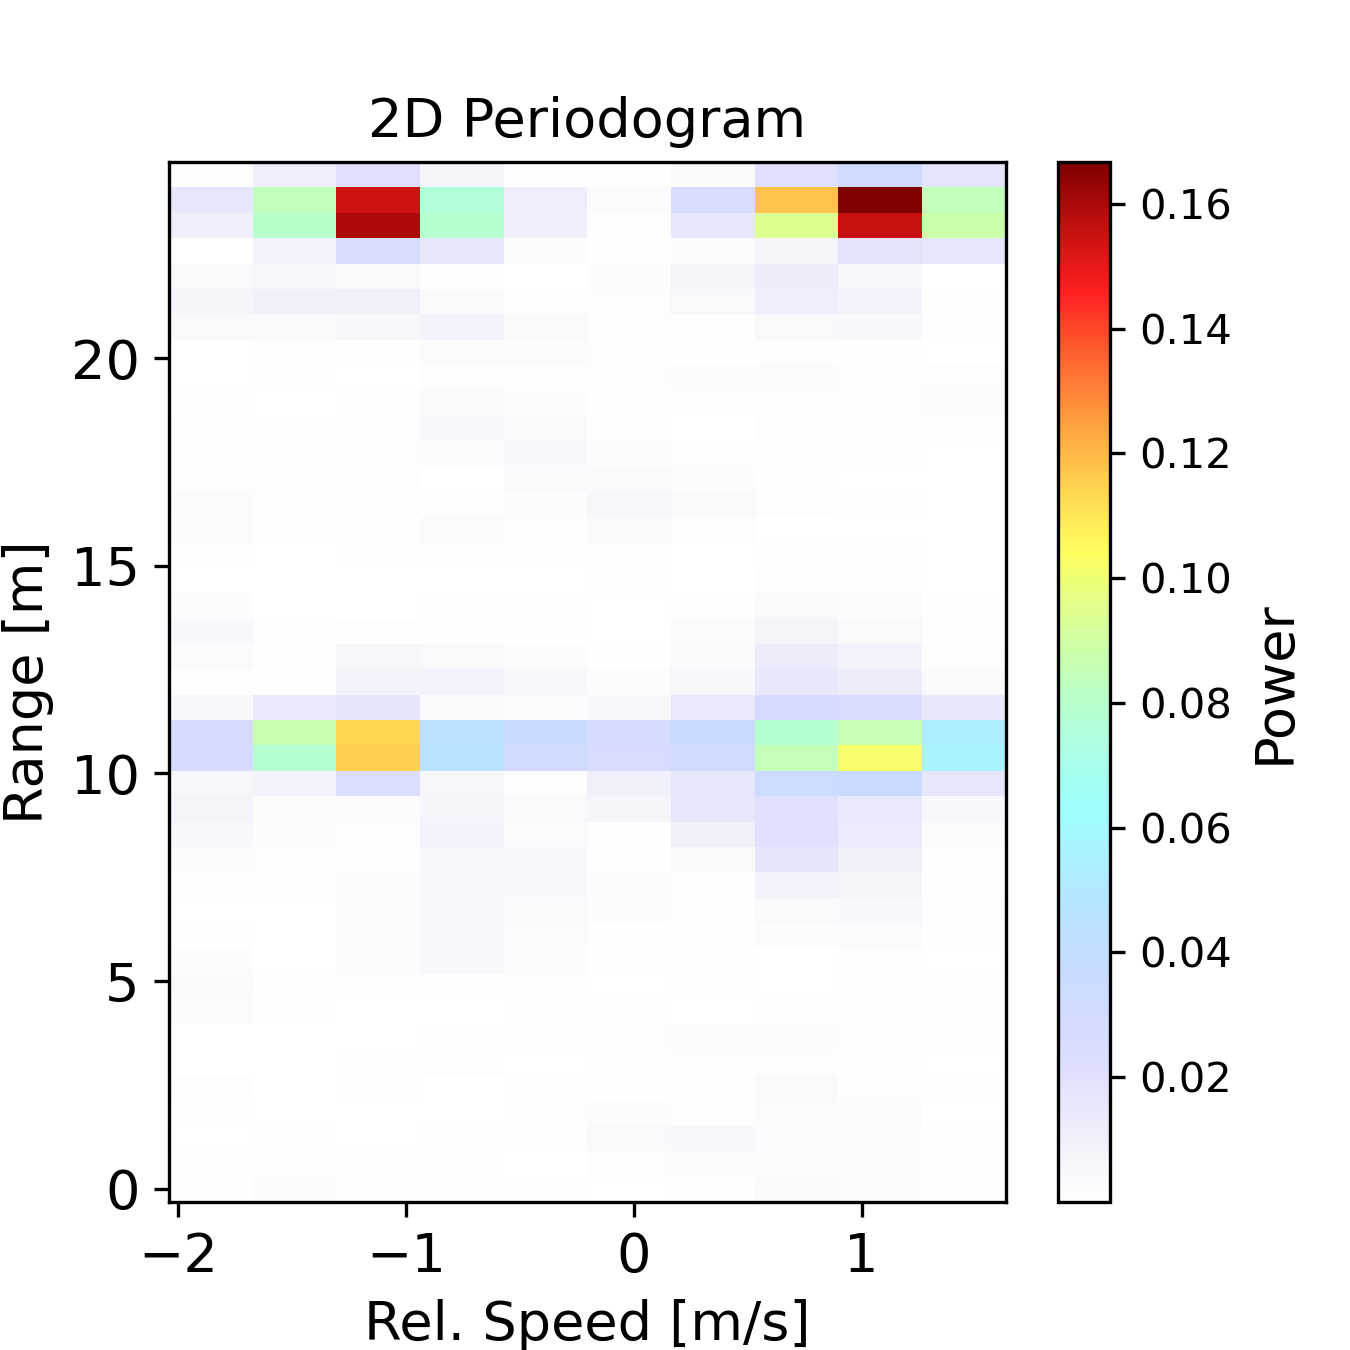
\includegraphics[scale=0.4]{Images/radar_detect_threshold/clutter/crap_ecac_static/clutter_ecac1.png}%
		}\hfill
		\subfloat[\footnotesize clutter removal using CRAP.\label{fig:Rad_crap_ecac_CRAP_static}]{
			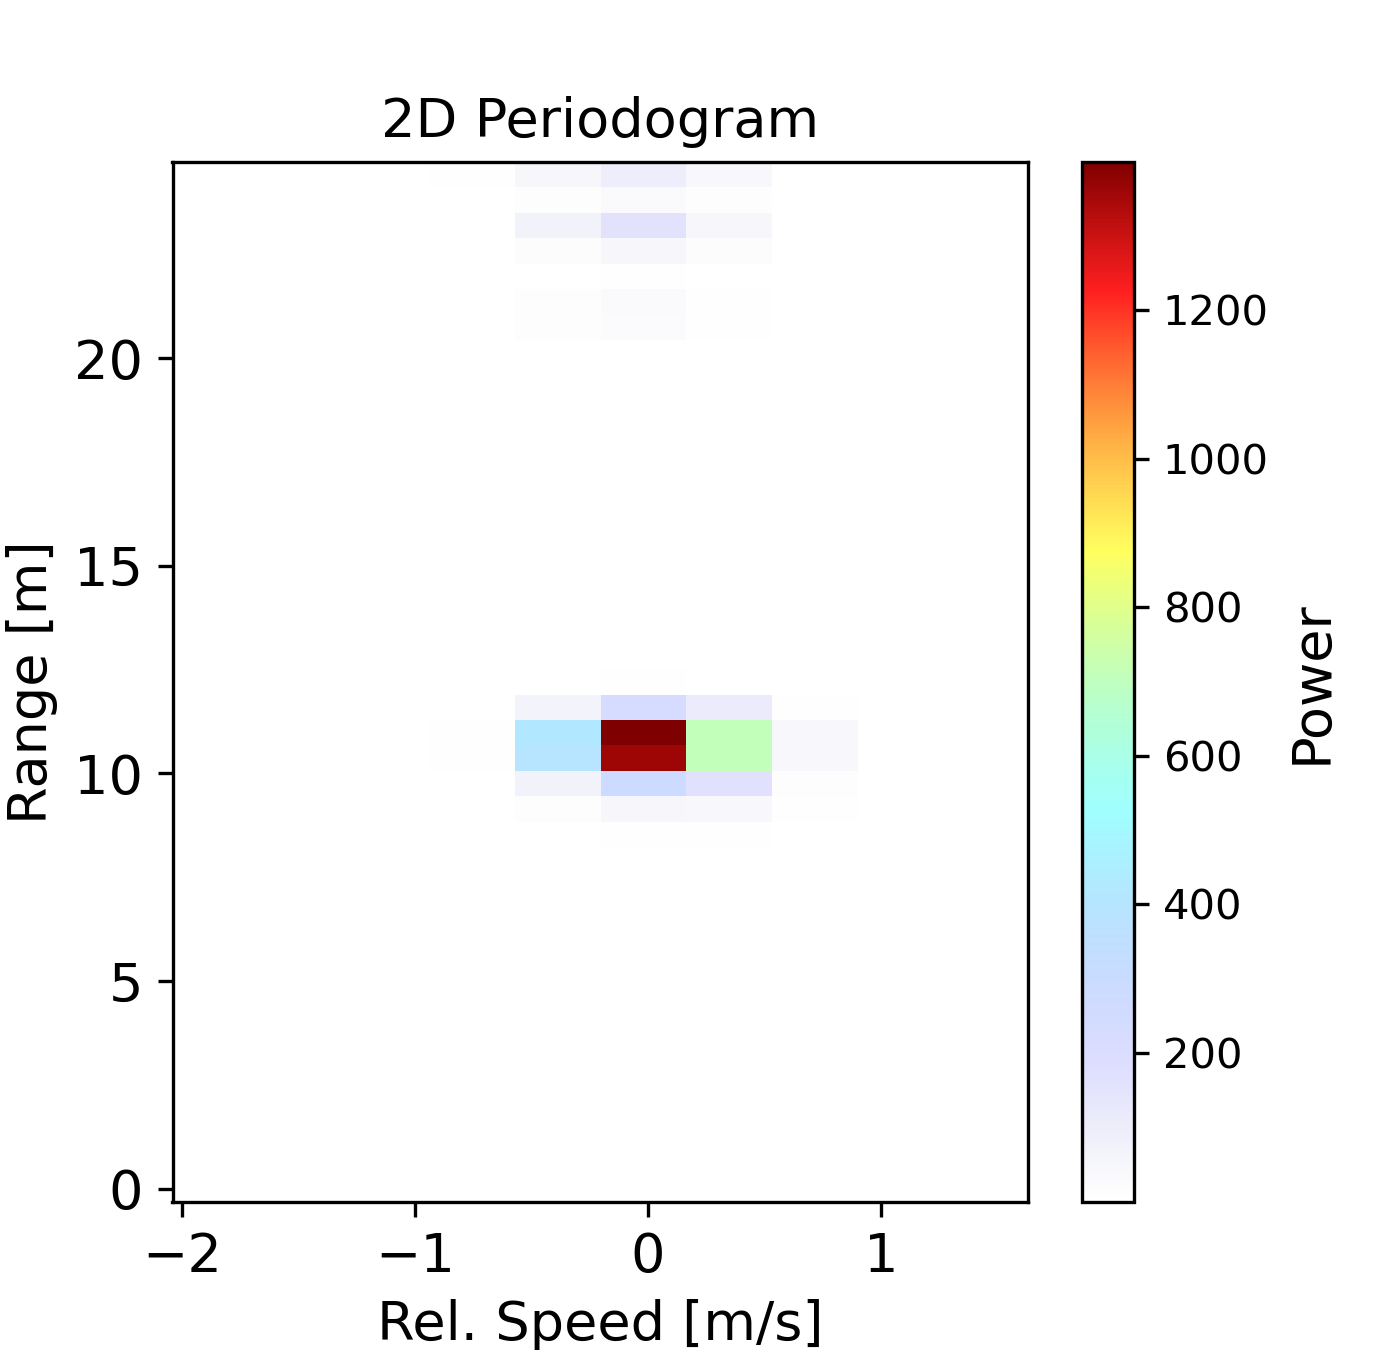
\includegraphics[scale=0.4]{Images/radar_detect_threshold/clutter/crap_ecac_static/clutter_crap1.png}
		}\newline
		
		\subfloat[\footnotesize no clutter removal, metal target at range of ca. 10 m moving at ca. 1 m/s.\newline Static clutter at ca. 23 m.\label{fig:Rad_crap_ecac_base_mov}]{%
			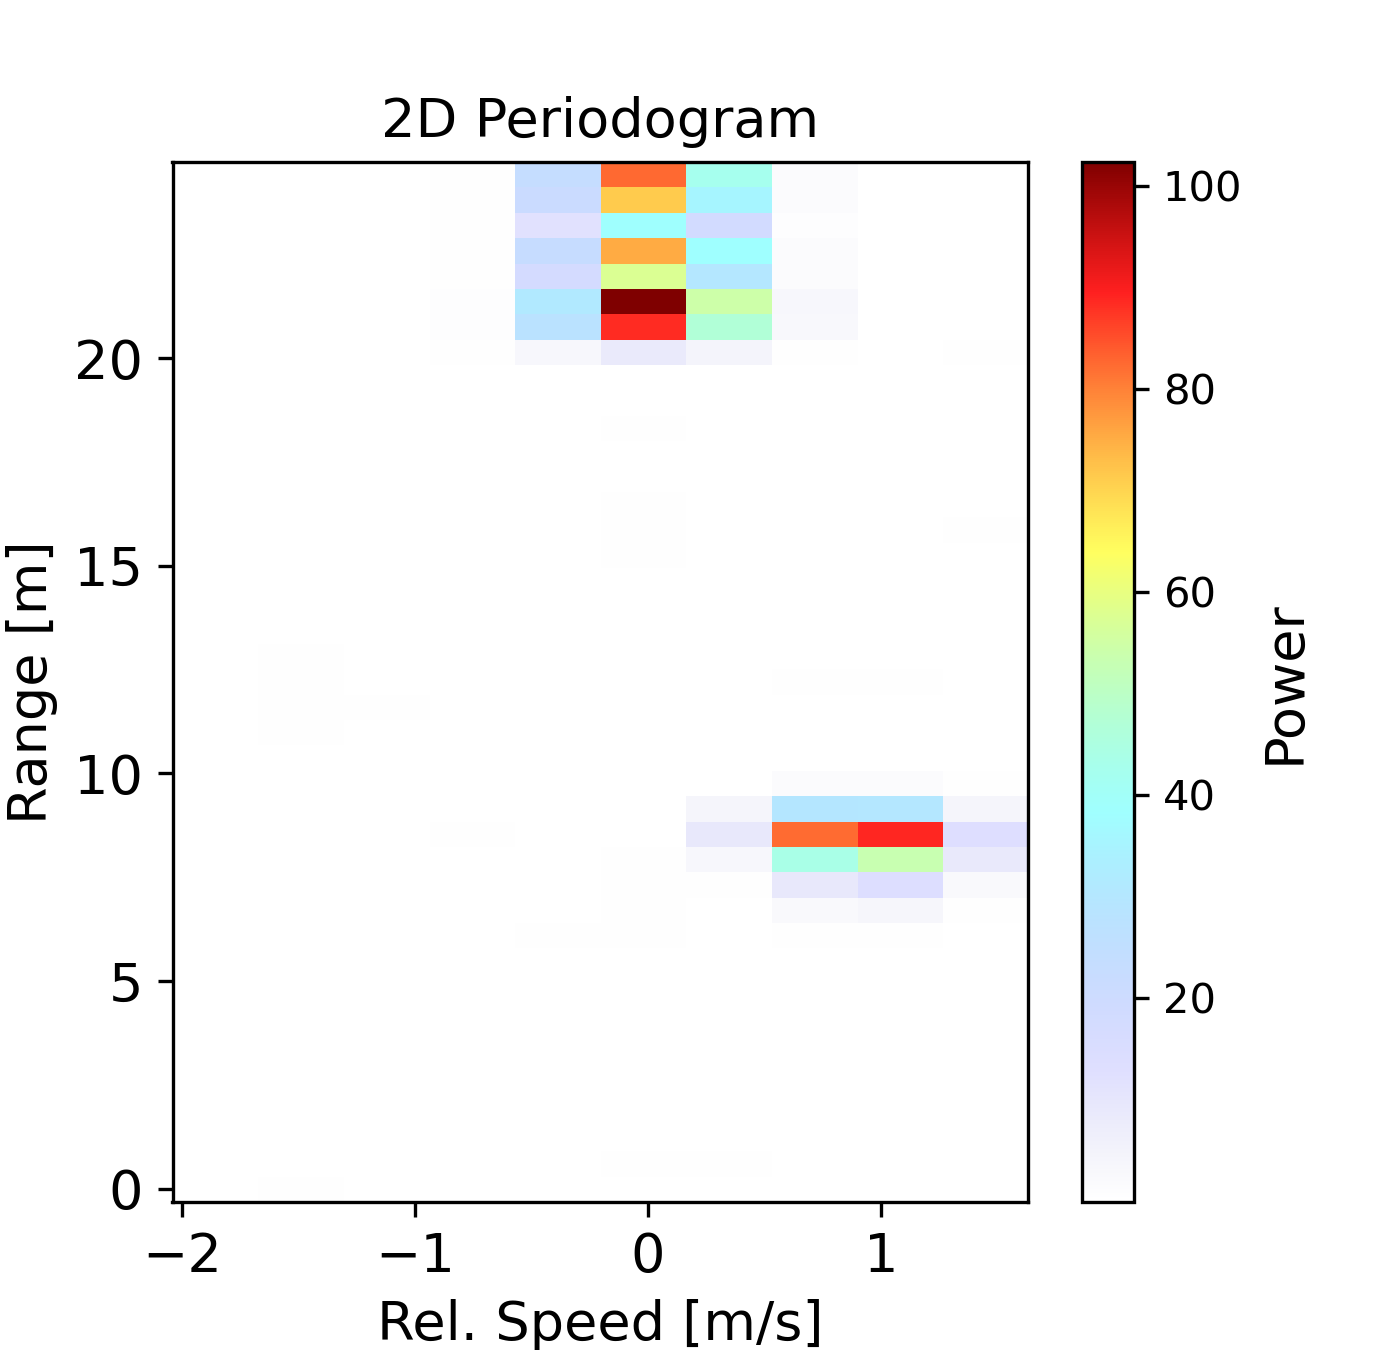
\includegraphics[scale=0.4]{Images/radar_detect_threshold/clutter/crap_ecac_mov/clutter_baseline_mov1.png}%
		}\hfill
		\subfloat[\footnotesize clutter removal with \newline ECA-C, moving target.\label{fig:Rad_crap_ecac_ECAC_mov}]{%
			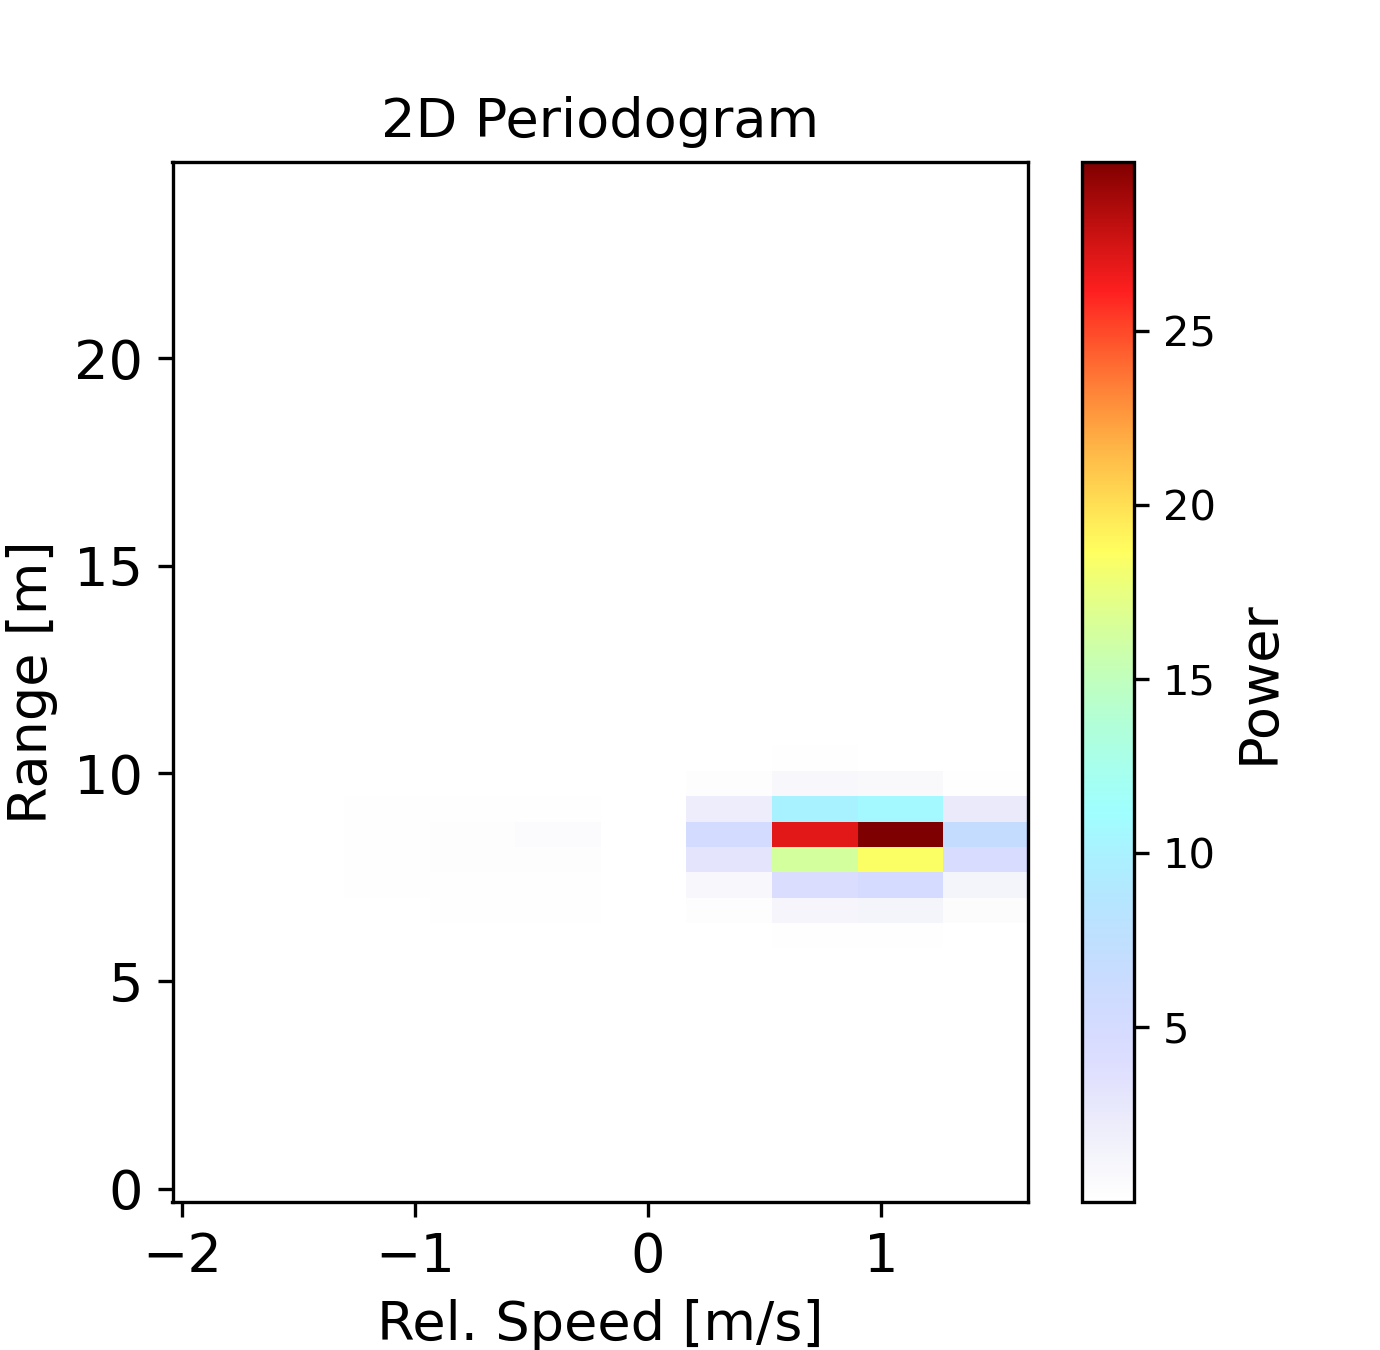
\includegraphics[scale=0.4]{Images/radar_detect_threshold/clutter/crap_ecac_mov/clutter_ecac_mov1.png}%
		}\hfill
		\subfloat[\footnotesize clutter removal using \newline CRAP, moving target. \label{fig:Rad_crap_ecac_CRAP_mov}]{%
			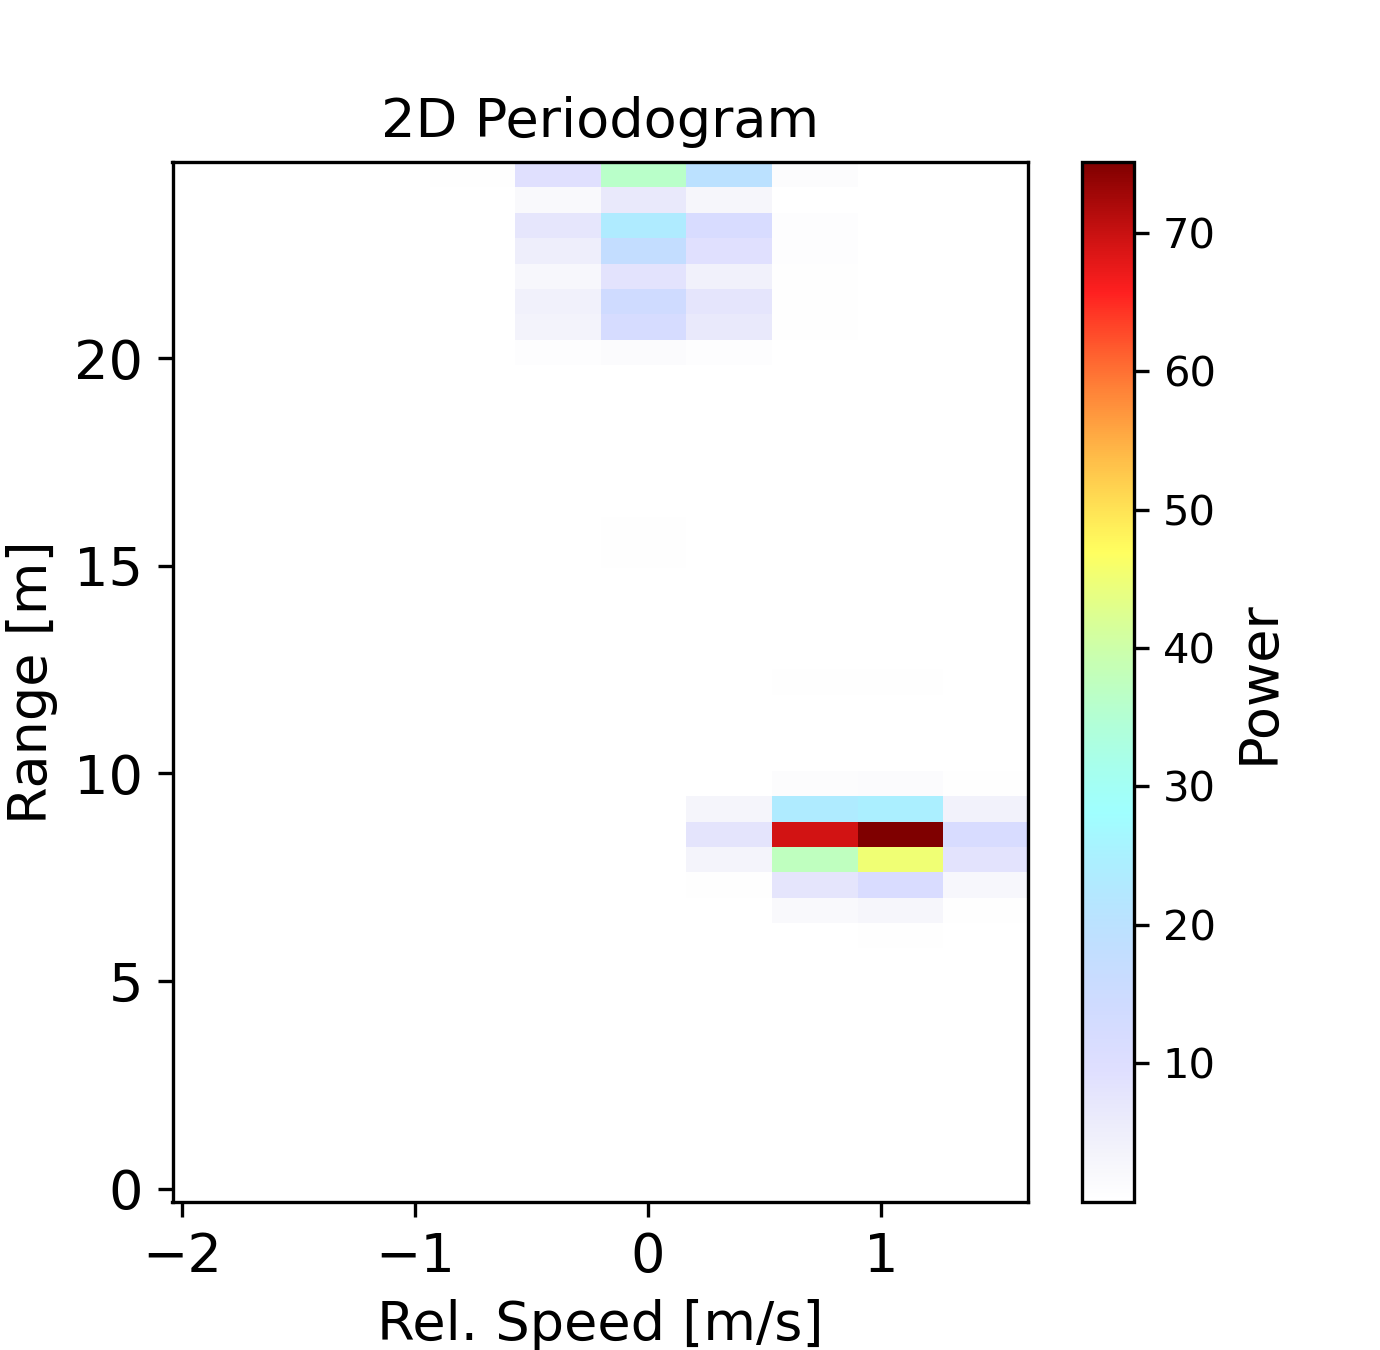
\includegraphics[scale=0.4]{Images/radar_detect_threshold/clutter/crap_ecac_mov/clutter_crap_mov1.png}%
		}
		\caption[]{\small Comparison of periodograms from sensing acquisitions obtained in NOKIA's indutrial test facility.
		Periodograms without clutter removal (left) are compared with those obtained after applying ECA-C (middle) and CRAP (right). It can be observed how ECA-C is able to clean the image from static clutter, albeit at the cost of losing information on static targets, as shown in \subref{fig:Rad_crap_ecac_ECAC_static}, whilst CRAP is able to retain the information.  }
		\label{fig:Rad_clutter_crap-ecac}
	\end{figure}
	
	\subsection{Clutter presence in NLOS}
	
	Even after applying clutter removal, static targets in the environment can still generate unwanted radar returns.
	In a NLOS sensing setup it is fairly easy to distinguish moving targets from the underlying noise floor.
	However, NLOS returns from static objects of interest will appear in the periodogram area where static clutter is more prevalent, as shown in Figure \ref{fig:Rad_clutter_comparison}.
	This makes the effective separation through radar thresholding and identification of the target difficult.

	\begin{figure}[H]
		\centering
		
		\subfloat[\label{fig:Rad_clutter_mov_target}]{%
			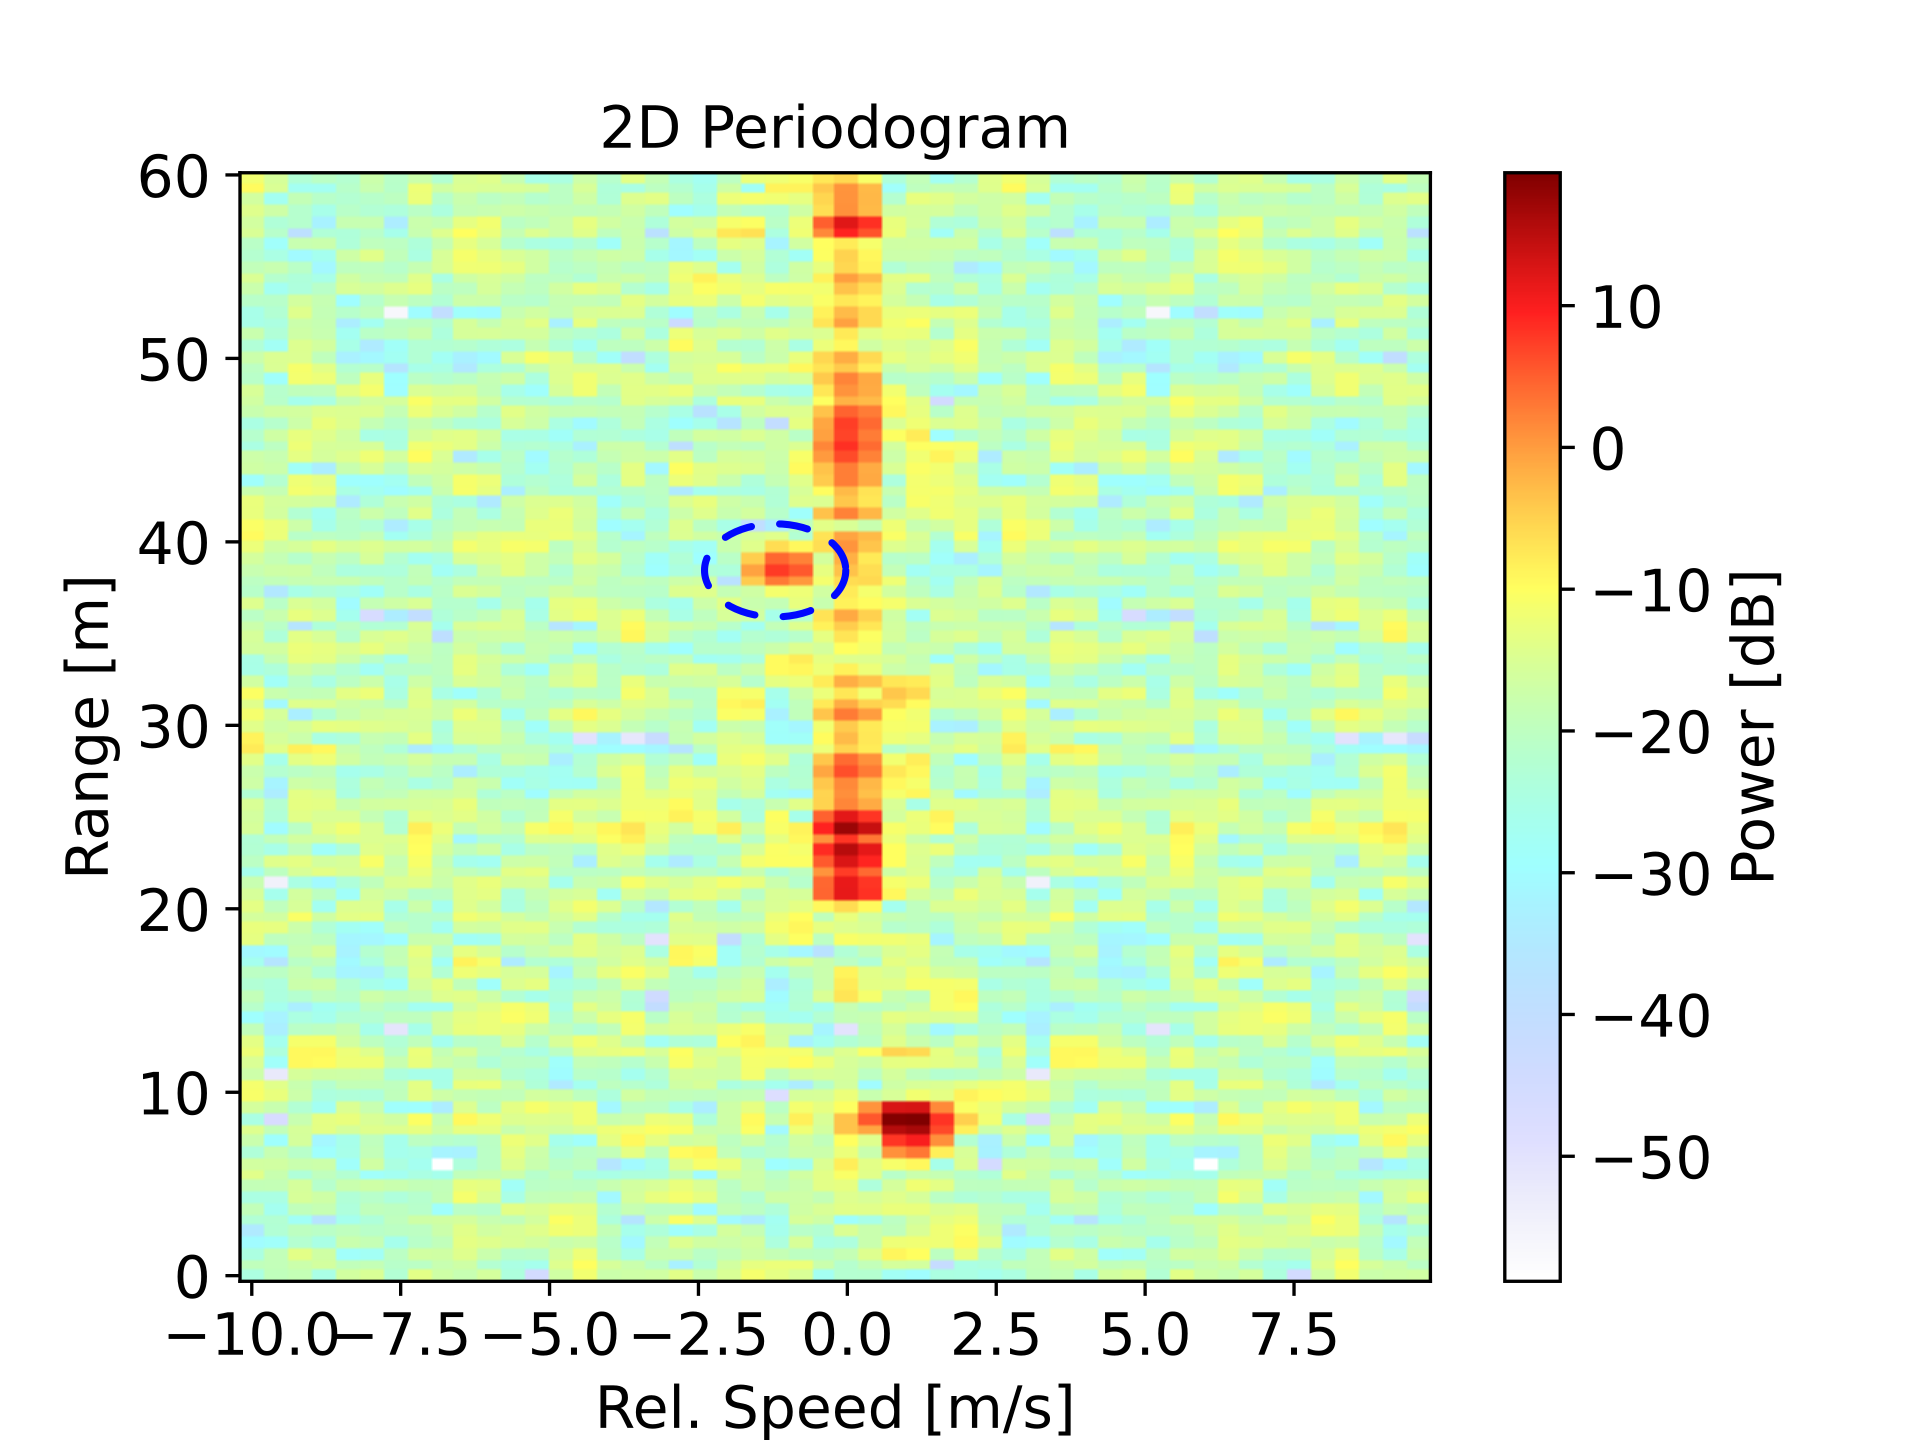
\includegraphics[scale=0.49]{Images/radar_detect_threshold/clutter/clutter_mov_target1.png}%
		}\hfill
		\subfloat[\label{fig:Rad_clutter_stat_target}]{%
			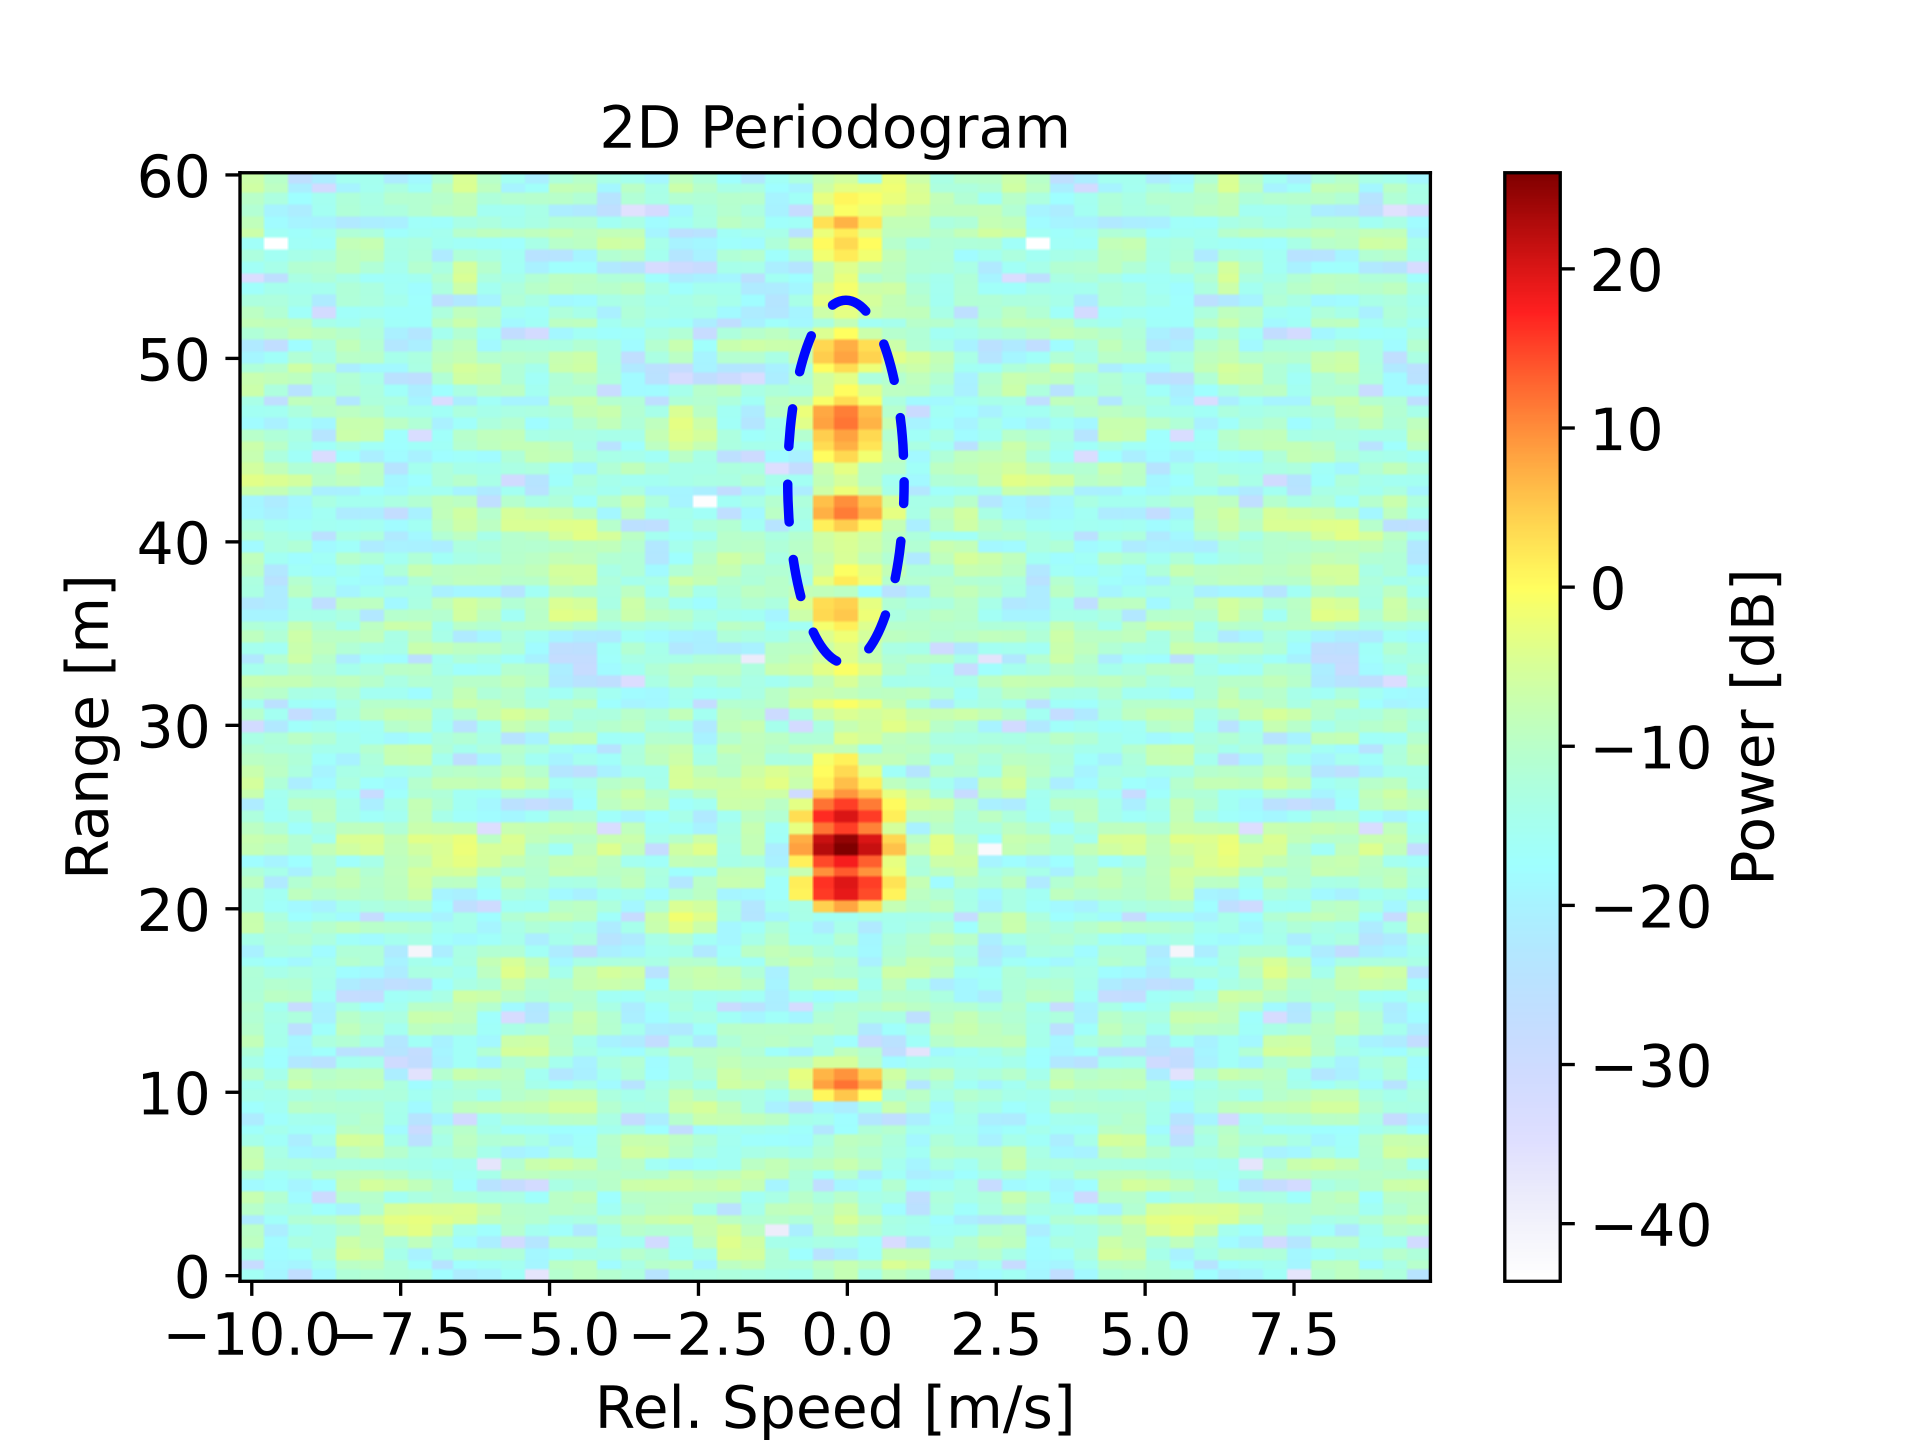
\includegraphics[scale=0.49]{Images/radar_detect_threshold/clutter/clutter_stat_target1.png}%
		}
		
		\caption[]{Periodograms with moving \subref{fig:Rad_clutter_mov_target}, and static \subref{fig:Rad_clutter_stat_target} targets in NLOS.
				Target is highlighted clearly when moving, while it appears as static clutter when it stops moving.}
		\label{fig:Rad_clutter_comparison}
	\end{figure}

	For intrusion detection purposes, it is sufficient to focus the radar search on moving targets. 
	Therefore, the static bins of the periodograms can be discarded for NLOS processing.
	
	\subsection{Line-of-sight and Non-line-of-sight separation}
	\label{sec:los_nlos_separation}
	
	
	
	In addition to clutter removal, calibration measurements provide valuable information for determining the distance threshold at which targets can be assumed to be in NLOS. 
	A portion of the calibration frames can be processed as radar frames, with a focus on the analysis of the zero-Doppler component.
	
	
	\begin{figure}[H]
		\centering
		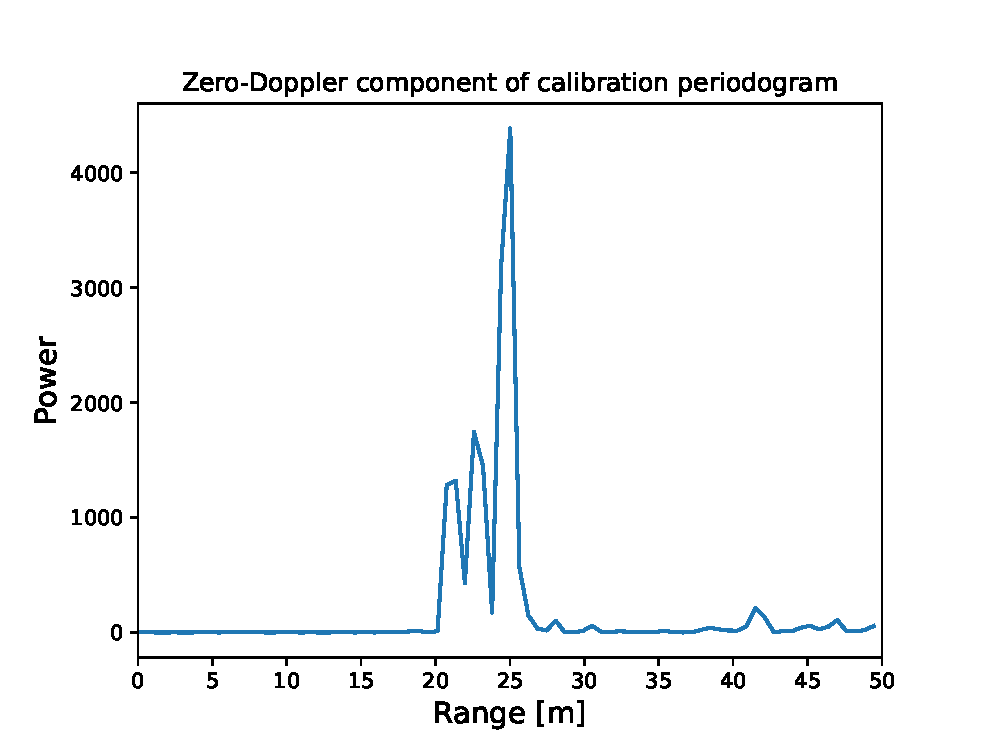
\includegraphics[width=0.6\textwidth]{Images/Test1/cali_static_per_t1.eps}
		\caption{Zero Doppler component of a periodogram generated from calibration measurements. It can be assumed that any returns detected beyond 25m from the system are generated from multiple reflections and should be considered as NLOS components. }
		\label{fig:Test1_cali_static_per}
	\end{figure}
	
	As can be seen in the figure \ref{fig:Test1_cali_static_per}, a target with large RCS is present approximately $25$ m from the system. It was assumed that any return associated with a range greater than $25$ m was generated by a signal reflected from the largest static target. The figure also indicates that static clutter has a larger amplitude for ranges greater than $25$ m compared to lower ranges. This is due to the part of the beam that is reflected from the wall towards the environment and the associated returns.
	
	The distance between the gNB and the reflector of the NLOS components was estimated during the calibration step by averaging over the available measures.
	
	\subsection{Modified periodogram}
	
	Figure \ref{fig:Rad_nlos_los_separation} highlights the regions of interest within the periodogram.
	The red area, which corresponds to static targets, is discarded. The periodogram is then divided horizontally into two regions, based on the range of the reflector for NLOS.
	
	\begin{figure}[H]
		\centering
		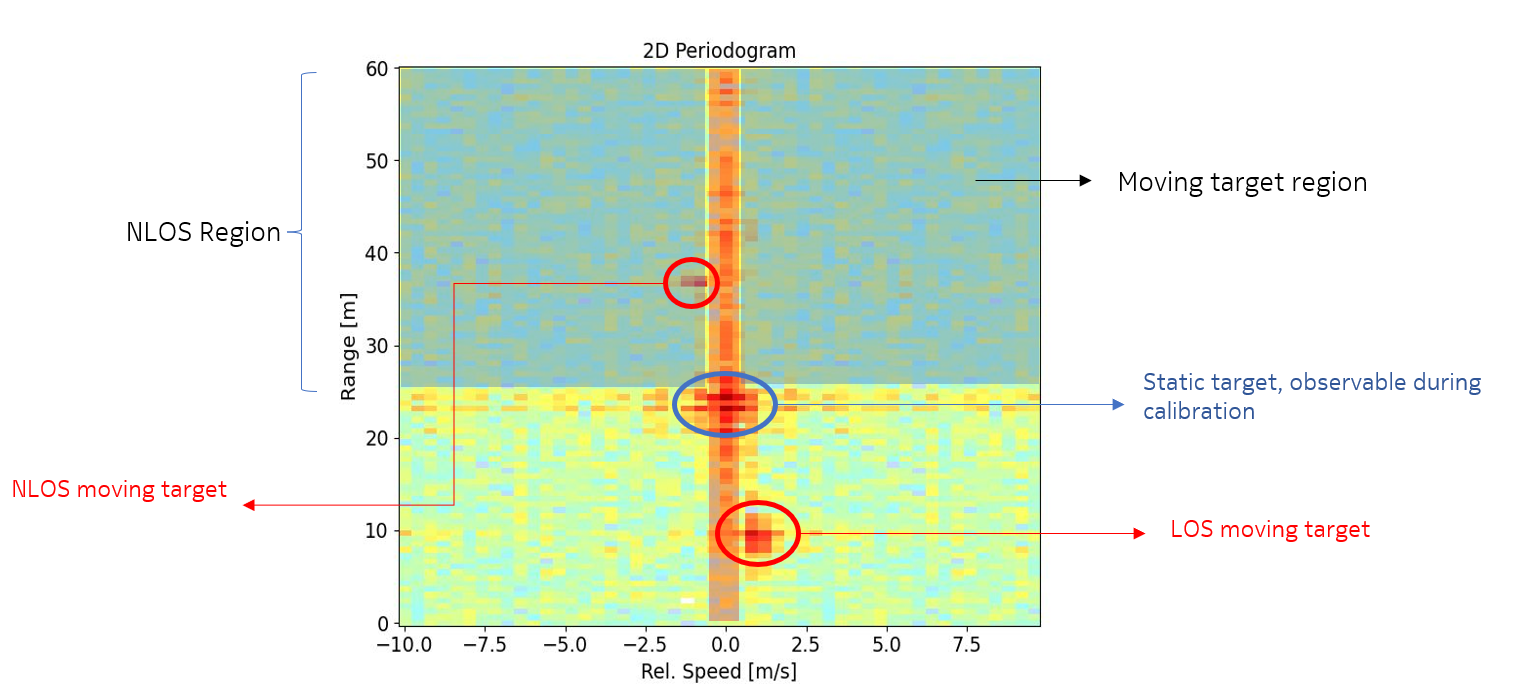
\includegraphics[width=1.1\textwidth]{Images/Test1/nlos-los-separation.png}
		\caption{Processed periodogram, separated in processing regions.}
		\label{fig:Rad_nlos_los_separation}
	\end{figure}
	
	
	After generating the periodogram, the processing phase can take into account this separation to process the NLOS section and LOS section separately.
	









% First Measurements
\chapter{Determining the presence of NLOS component}

The first set of practical measurements was carried out in order to determine the presence and observe the characteristics of the non-line-of-sight component of the signal. 

\section{Measurements setup}

The measurements were obtained using Nokia's sensing proof-of-concept described in section \ref{sec:intro-PoCarchitecture}. The system was mounted in an indoor scenario, with the receiver positioned at a height of $5,12$ m. The transmitter was positioned towards an open indoor area, located approximately 23 metres away from a warehouse rack (which was in front of a wall) and a cargo door.
The objective was to obtain a non-line-of-sight measurement by reflecting the signal on the wall and subsequently on a moving target. 

The tests were carried out using:

\begin{enumerate}
	\item A human target.
	\item A strong reflector (large metal cabinet with flat surfaces).
\end{enumerate}

The direction (azimuth $\theta$ and elevation $\varphi$) of the transmitted beam was fixed for the whole measurement.

Before each test, a short calibration measure is performed, which includes only the static elements of the scenario. The calibration data will be used in the post-processing steps for subspace-based clutter removal with the CRAP method  \cite{Henninger_Mandelli_Grudnitsky_Wild_Brink_2023}. 


% TODO: check if axes are needed
\begin{figure}[H]
	\centering
	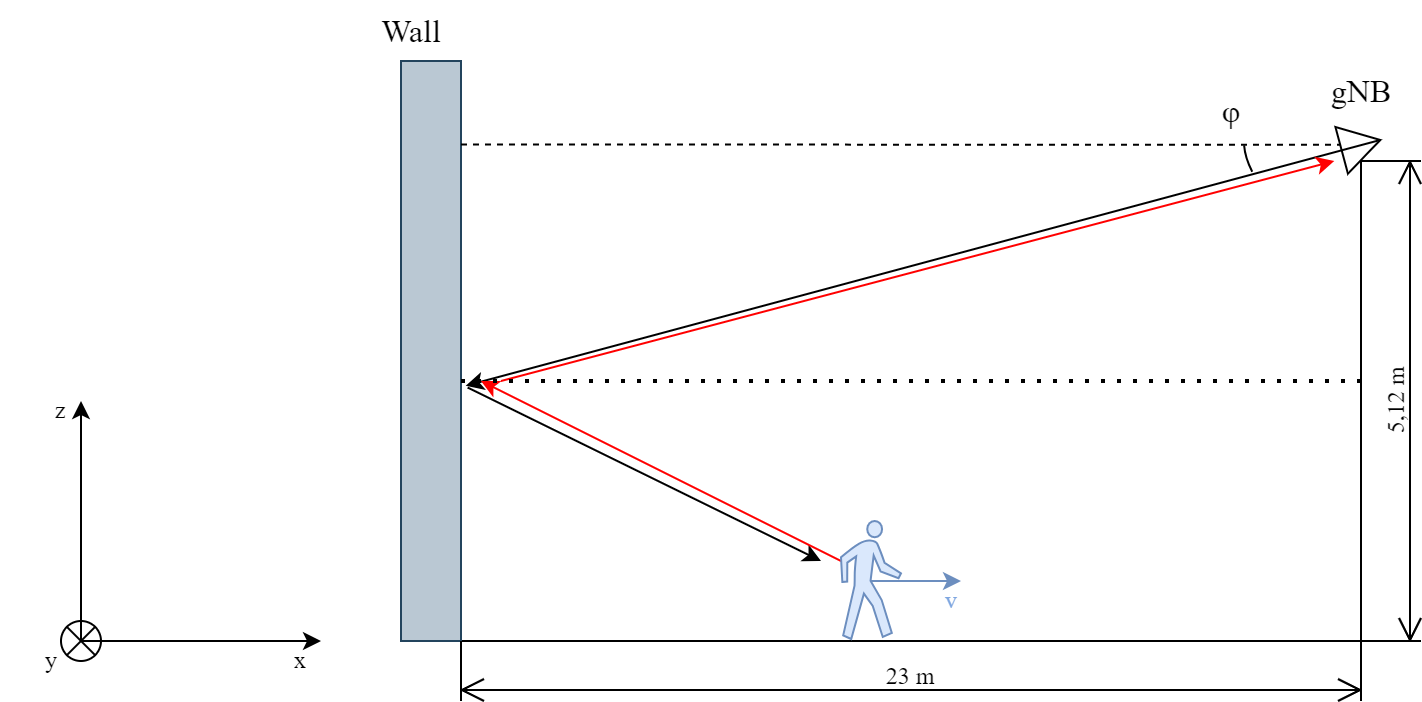
\includegraphics[width=0.9\textwidth]{Images/Test1/base-lateral_view}
	\caption{Zero Doppler component of a periodogram generated from calibration measurements.}
	\label{fig:Test1_base-lateral_view}
\end{figure}

\section{Moving target without obstructions}

The OFDM radar system will be able to determine the range and radial speed component (the angle of arrival AOA is fixed). During the initial measurement the antenna boresight was directed perpendicular to the wall,while the target moved radially between the transmitter and reflector.

\begin{figure}[H]
	\centering
	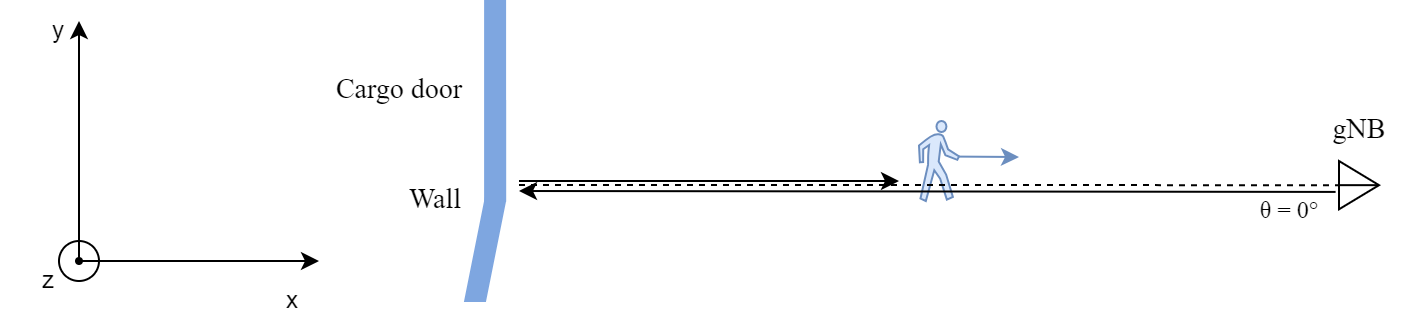
\includegraphics[width=0.9\textwidth]{Images/Test1/base-top_view}
	\caption{Top view of measurement scenario.}
	\label{fig:Test1_base-top_view}
\end{figure}


Beam elevation was chosen to be as high as possible in order to avoid line-of-sight from the transmitted beam's main lobe. Beam parameters are shown in table \ref{table:Test1TXBeamParams}.


% TODO: check if it's the case of adding something to the table
\begin{table}[H]
	%\caption*{\textbf{Title of Table (optional)}}
	\centering 
	\begin{tabular}{|p{9em} c c |}
		\hline
		\rowcolor{bluepoli!40} % comment this line to remove the color
		\textbf{} & \textbf{$\theta$ (azimuth [\textdegree])} & \textbf{$\varphi$ (elevation [\textdegree])} \T\B \\
		\hline \hline
		$\textbf{TX beam}$ & $\approx 0$ & $4$ \T\B \\
		
		\hline
	\end{tabular}
	\\[10pt]
	\caption{Transmitted beam parameters for initial measurements.}
	\label{table:Test1TXBeamParams}
\end{table}

Since only the radial component of speed can be measured, the aim of the test was to maximize this component in order to analyze the characteristics of the signal generated from the reflection.

\subsection{Line-of-sight and non-line-of-sight separation}

In addition to clutter removal, calibration measurements provide valuable information for the determination of the distance threshold at which targets can be accurately classified as NLOS. Certain calibration frames can be processed as radar frames, with a focus on analyzing the zero-Doppler component.
	

\begin{figure}[H]
	\centering
	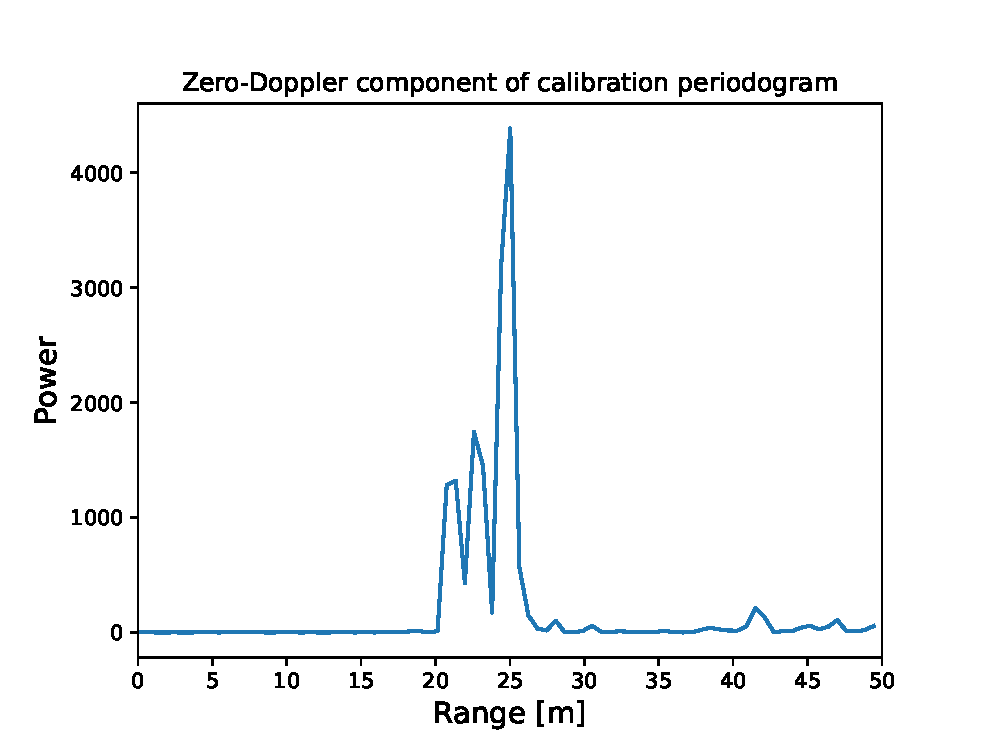
\includegraphics[width=0.6\textwidth]{Images/Test1/cali_static_per_t1.eps}
	\caption{Zero Doppler component of a periodogram generated from calibration measurements.}
	\label{fig:Test1_cali_static_per}
\end{figure}

As can be seen in the figure \ref{fig:Test1_cali_static_per}, a large target is present approximately $23$ m from the system. It was assumed that any target return associated with a range greater than $23$ m was generated by a signal reflected from the main target. The figure also indicates that static clutter has a larger amplitude for ranges greater than $23$ m compared to lower ranges. This is due to the part of the beam that is reflected from the wall towards the environment.

Identifying static NLOS targets from the background was challenging due to the high power of clutter components in the NLOS region, even after clutter removal. However, it was easier to detect obscured targets by analyzing the moving target region of the periodogram. The separation of the regions is highlighted in figure \ref{fig:Test1_nlos_los_separation}.

\begin{figure}[H]
	\centering
	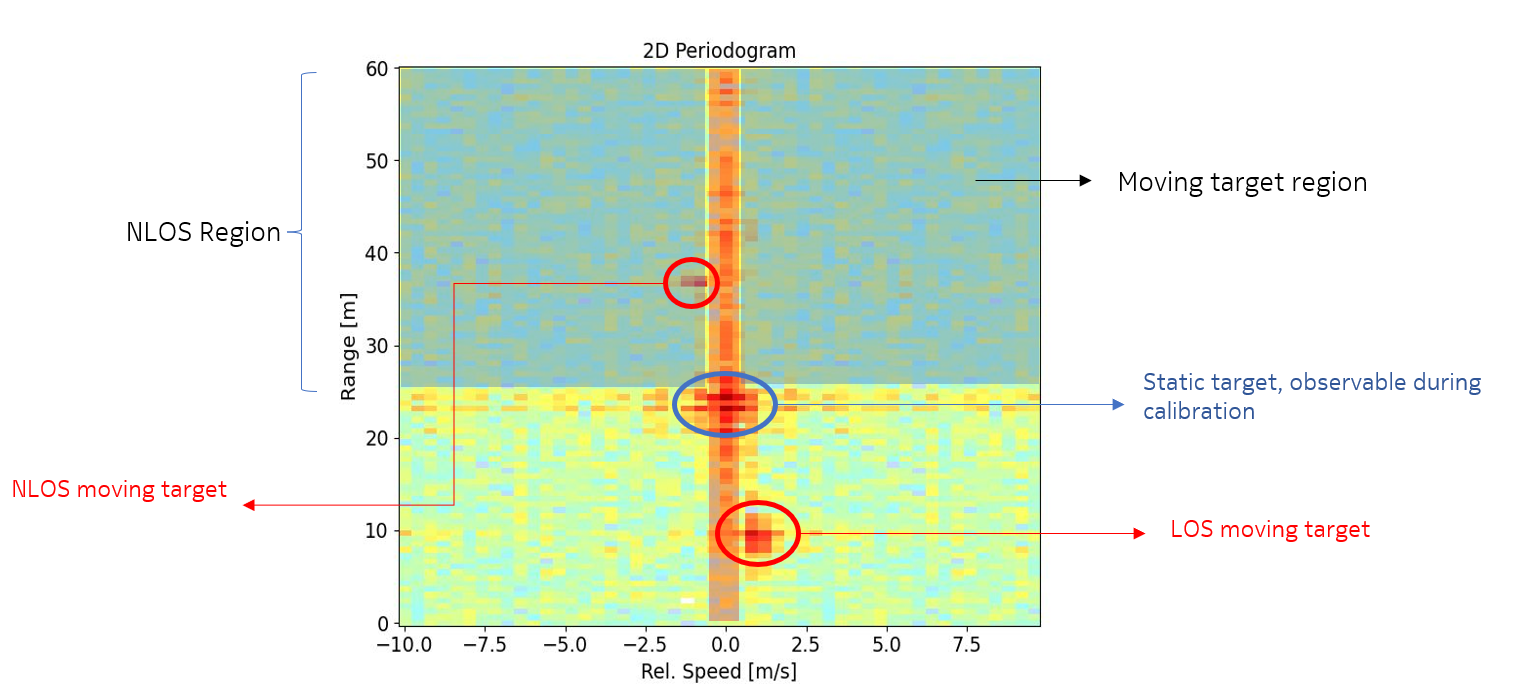
\includegraphics[width=0.9\textwidth]{Images/Test1/nlos-los-separation.png}
	\caption{Processed periodogram, separated in processing regions.}
	\label{fig:Test1_nlos_los_separation}
\end{figure}


After the periodogram has been generated, this separation can be taken into account in the post-processing phase to process the NLOS section separately from the LOS one.

\subsection{Line-of-sight component as ground truth}

Due to the rather large beamwidth of the system, $\pm$7\textdegree\hspace{1pt} in azimuth and elevation, and its sidelobes, the measurement observed the presence of a LOS target return in addition to the expected NLOS one generated by reflection.

During the measurement, the direct component was always visible as no other obstacle was positioned in the scene. It was then decided to use this component and the knowledge of the target geometry to obtain an estimate of the position and velocity of the NLOS return. This estimate was used to check if any of the detected peaks corresponded to the moving target.

\textit{Detection rate} was defined as the metric used to evaluate the experiment: if the speed and range of the detected NLOS target matched the expected value calculated from the LOS component detection, it was considered positive.
The detection rate was then obtained as the ratio between the number of frames in which the NLOS component was above the threshold and the total number of frames in which the LOS component was detected.

\subsection{Processing of the NLOS region}

After defining the two regions of interest from the periodogram, peak detection is conducted separately. A standard strongest peak search is performed for the LOS region, and accurate range and velocity measurements are obtained after interpolation of the adjacent bins.

\begin{figure}[H]
	\centering
	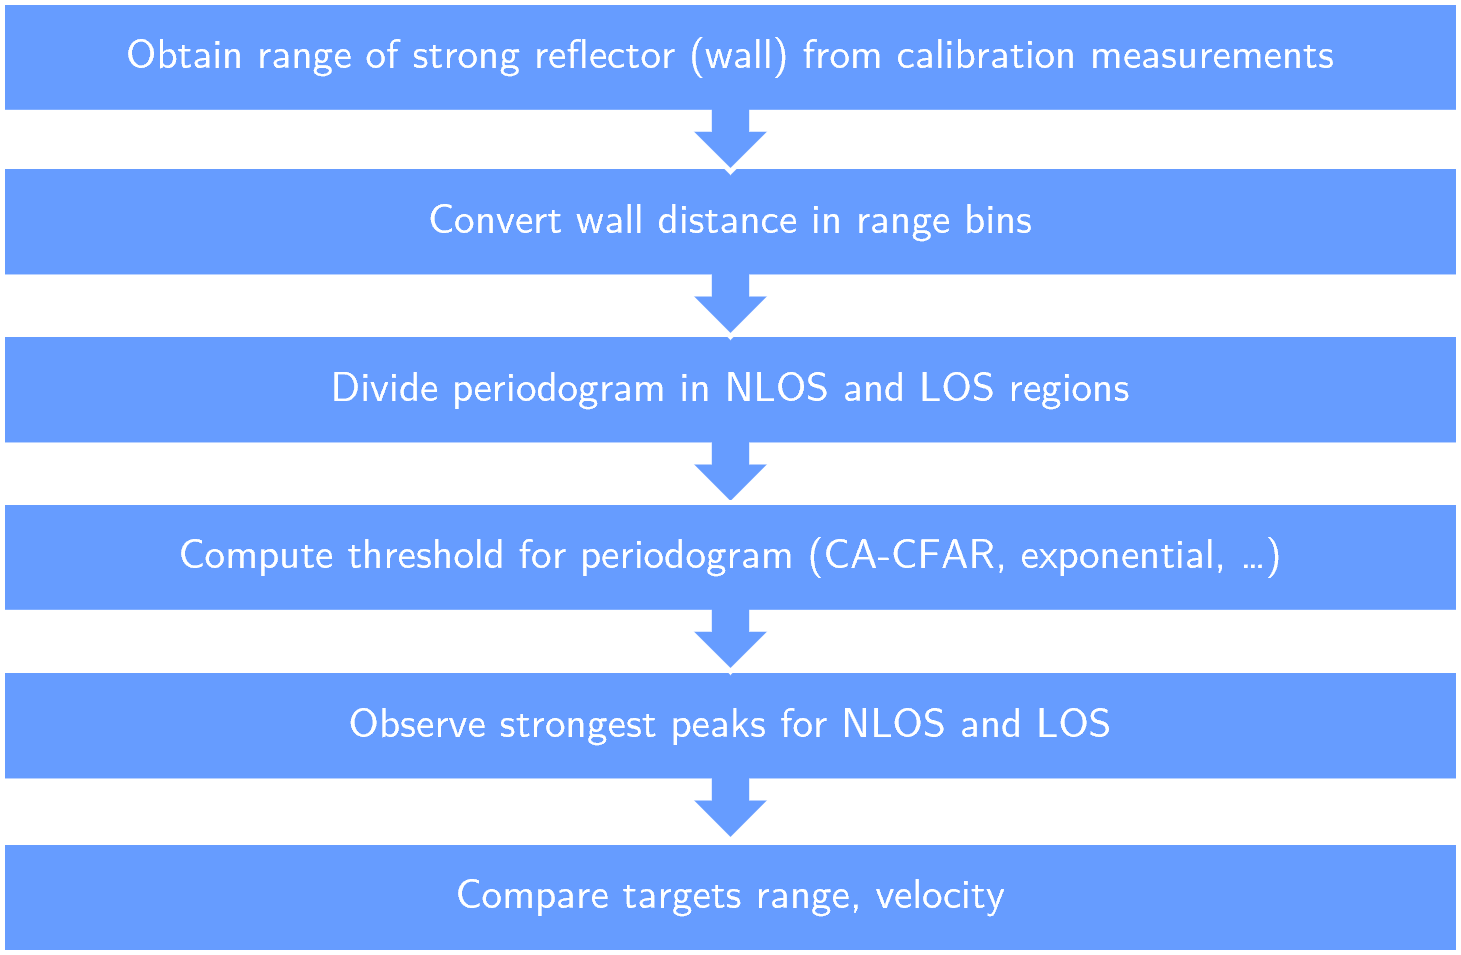
\includegraphics[width=0.9\textwidth]{Images/Test1/NLOS-proc-pipeline.png}
	\caption{Periodogram processing pipeline used for detection tests.}
	\label{fig:Test1_NLOS-proc-pipeline}
\end{figure}


Due to the presence of strong clutter components in the bins close to zero speed, the target search in the NLOS region was performed neglecting this part of the periodogram.

The full process for the experiment is summarized in figure \ref{fig:Test1_NLOS-proc-pipeline}.

The detection strategy chosen was CA-CFAR, which utilized a square contribution window and a probability of false alarm $p_{\text{FA}} = 10^{-6}$. The size of the CA-CFAR window was set depending on the width of the target in speed bins, which depended on number of processed frames and OFDM sampled symbols.  

\subsection{Observed detection rate}

The results were obtained with the different frame processing strategies presented in chapter \ref{chap:TDD pattern of the OFDM frame}. Target detection was carried out considering the \textit{n}-strongest peaks and comparing them against the LOS data.

\begin{figure}[H]
	\centering
	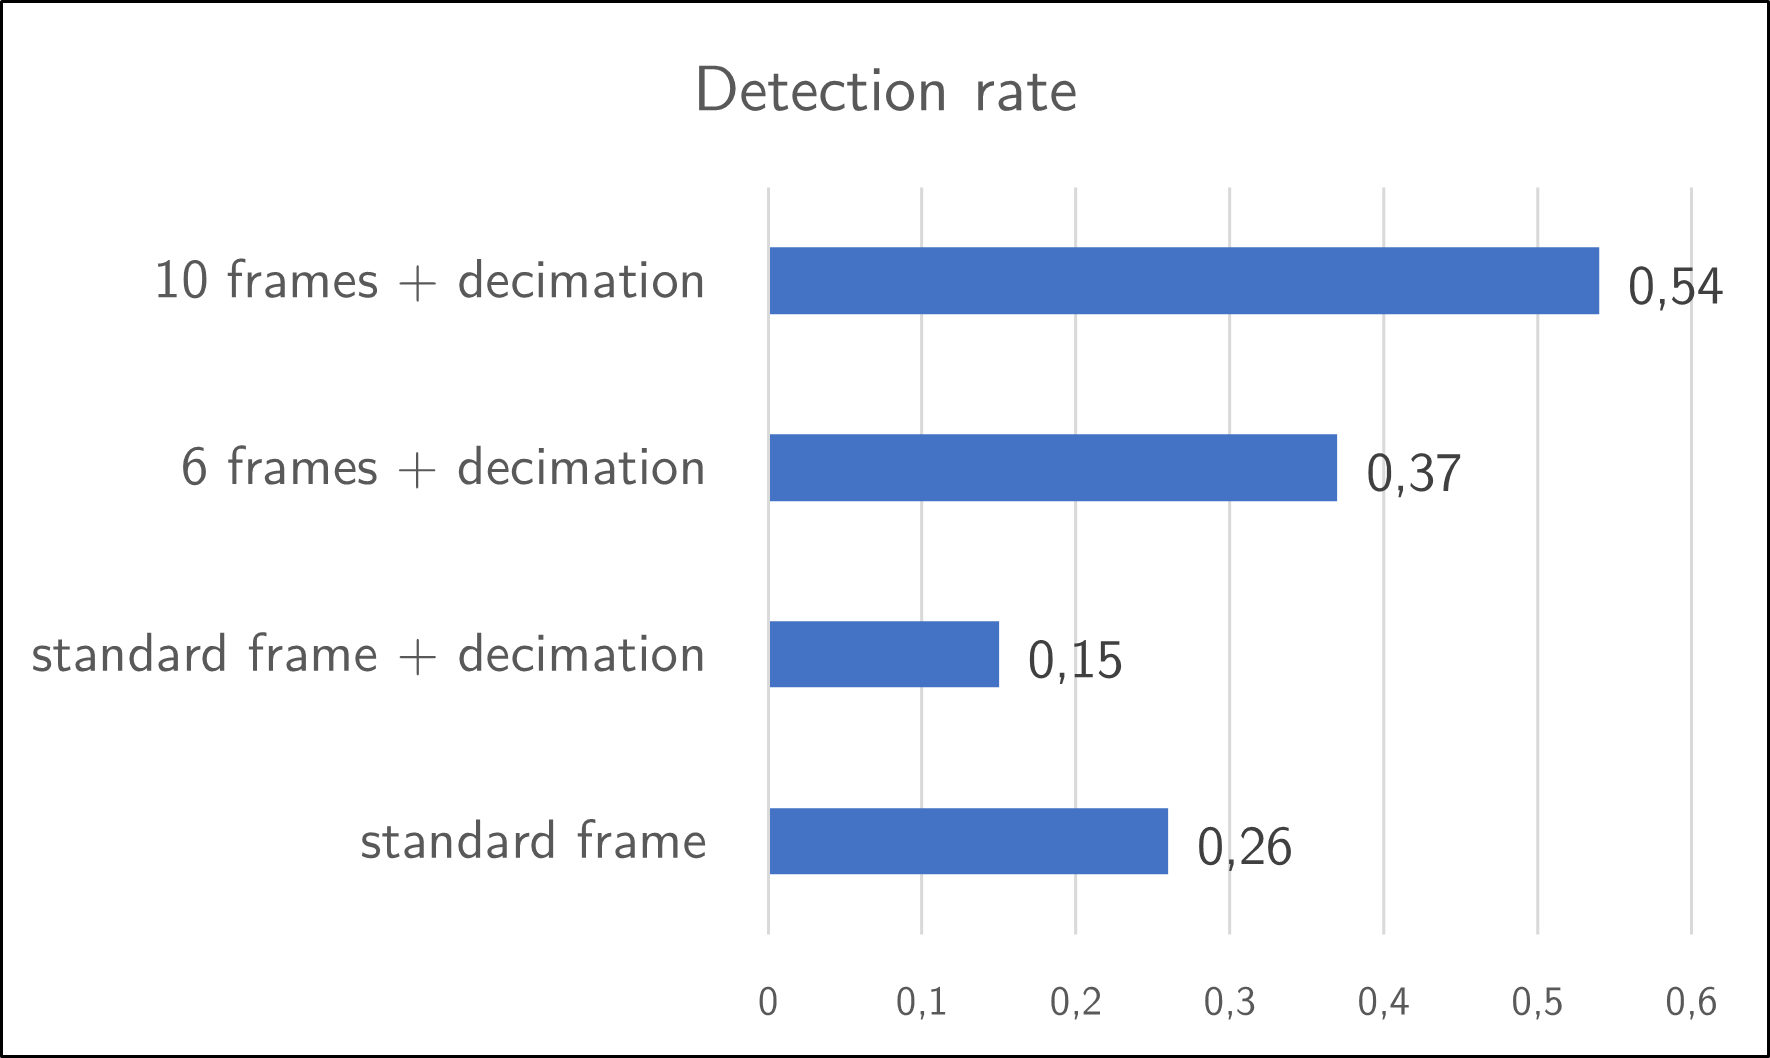
\includegraphics[width=0.7\textwidth]{Images/Test1/detect_hist.png}
	\caption{Detection rate observed for human target in mixed LOS/NLOS measurement.}
	\label{fig:Test1_detect_hist}
\end{figure}

Using a larger time-aperture significantly increased the detection rate due to the improved speed resolution. However, it may cause range spreading issues, particularly for fast targets. This phenomenon is not a significant drawback in NLOS sensing since the system's primary objective is target detection rather than precise tracking and positioning.

It was observed that the NLOS target return was not the strongest return in the majority of cases, with lower power due to noise, spectral artefacts or channel fading.

The obtained detection rate considered the whole measure: frames where the target changed direction and was therefore static, or presented a low-speed component were considered. Processing of these time-instants means that the effective detection rate measured only when target is moving will be higher.

% TODO: change picture with higher resolution one
\begin{figure}[H]
	\centering
	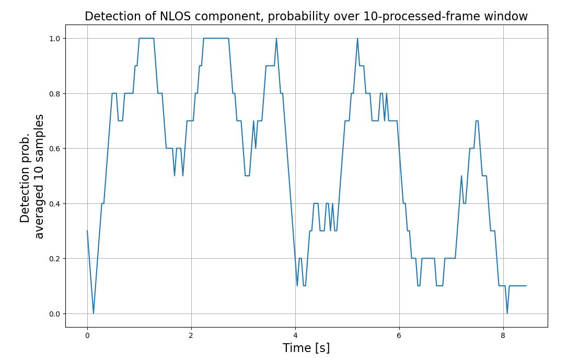
\includegraphics[width=0.7\textwidth]{Images/Test1/moving_avg.png}
	\caption{Detection rate observed for human target in mixed LOS/NLOS measurement.}
	\label{fig:Test1_moving_avg}
\end{figure}




\chapter{Outlook and Conclusion}

In summary, this thesis investigated the integration of sensing and communication capabilities in the context of 5G Advanced and 6G wireless systems. 
The main objective of this work was to explore the potential of non-line-of-sight (NLOS) sensing techniques and their applications in integrated radar systems. 

The results obtained from processing real-word measurements suggest that use cases with NLOS conditions should be considered in future studies in ISAC.
With a focus on intrusion detection this work suggests that, with further analysis of the NLOS radar returns and the corresponding processing techniques, NLOS sensing at mmWave is possible.

The main contributions of this work can be summarized as:

\begin{itemize}
	\item Real-word NLOS sensing trials and identification of challenges due to communication requirements.
	\item Proposal of CSI processing approaches for avoiding unwanted replicas in the periodogram.
	\item Definition of requirements for NLOS sensing and validation on measurements from the prototype.
\end{itemize}

Looking forward future developments, several challenges and research directions need to be explored:

\begin{itemize}
	\item \textbf{Algorithms for NLOS intrusion detection:} The promising detection results presented in this work suggest that true NLOS detection is possible, without the use of additional systems.
	\item \textbf{Multiple target detection:} The effect of multiple entities moving in an obscured environment still needs to be explored through new measurements and processing techniques.
	\item \textbf{Target differentiation and classification:} Solving the presence of replicas and spectral artifacts in the periodogram can open up the possibility of new processing methods that can be used for target classification in NLOS. Some promising examples are as micro-Doppler signatures, optical flow of moving peaks in the periodogram and machine vision.
	\item \textbf{Overcoming limitations due to blanks in the CSI:} More research has to be done for tackling the problem of empty slots within the CSI matrix, caused by communication requirements such as TDD transmission pattern and allocation of unused OFDM symbols. This is especially important considering the energy efficiency requirements for next-gen cellular networks.
\end{itemize}


%-------------------------------------------------------------------------
%	BIBLIOGRAPHY
%-------------------------------------------------------------------------

\addtocontents{toc}{\vspace{2em}} % Add a gap in the Contents, for aesthetics
% \bibliographystyle{IEEEtran}
\bibliography{Thesis_bibliography} % The references information are stored in the file named "Thesis_bibliography.bib"

%-------------------------------------------------------------------------
%	APPENDICES
%-------------------------------------------------------------------------

\cleardoublepage
\addtocontents{toc}{\vspace{2em}} % Add a gap in the Contents, for aesthetics
%\appendix
% \chapter{Appendix A}
%If you need to include an appendix to support the research in your thesis, you can place it at the end of the manuscript.
%An appendix contains supplementary material (figures, tables, data, codes, mathematical proofs, surveys, \dots)
% which supplement the main results contained in the previous chapters.


% ABBREVIATIONS
\chapter*{Abbreviations} % You have to include a chapter for your list of symbols (

\begin{table}[H]
    \begin{tabular}{ll}
    	AWGN & additive white Gaussian noise \\[2px]
    	CA-CFAR & cell-averaging CFAR \\[2px]
    	CFAR & constant false-alarm rate \\[2px]
    	CP & cyclic prefix \\[2px]
    	CSI & channel state information \\[2px]
    	CUT & cell under test \\[2px]
    	DL & downlink \\[2px]
    	DSP & digital signal processing \\[2px]
    	FMCW & frequency-modulated continuos-wave \\[2px]
    	ISI & inter-symbol interference \\[2px]
        LTE & long-term evolution \\[2px]
        LOS & line-of-sight \\[2px]
        MIMO & multiple-input multiple-output \\[2px]
        NLOS & non-line-of-sight \\[2px]
        NR & new radio\\[2px]
        OFDM & orthogonal frequency division multiplexing \\[2px]
        PSD & power spectral density  \\[2px]
        RCS & radar cross section \\[2px]
        SNR & signal-to-noise ratio \\[2px]
        UL & uplink \\[2px]
        
        
    \end{tabular}
\end{table}

% LIST OF FIGURES
\listoffigures

% LIST OF TABLES
\listoftables

% LIST OF SYMBOLS
% Write out the List of Symbols in this page
\chapter*{List of Symbols} % You have to include a chapter for your list of symbols (
\begin{table}[H]
    \centering
    \begin{tabular}{lll}
        \textbf{Variable} & \textbf{Description} & \textbf{SI unit} \\\hline\\[-9px]
        $\bm{u}$ & solid displacement & m \\[2px]
        $\bm{u}_f$ & fluid displacement & m \\[2px]
        $\bm{c}_0$ & speed of light & m/s \\[2px]
        $\bm{f}_C$ & carrier frequency & Hz \\[2px]
    \end{tabular}
\end{table}

% ACKNOWLEDGEMENTS
\chapter*{Acknowledgements}
Here you might want to acknowledge someone.

\cleardoublepage


\end{document}